\documentclass[11pt]{article}

\usepackage[T1]{fontenc}
\usepackage[utf8]{inputenc}
\usepackage{lmodern}
\usepackage{microtype}
\usepackage[a4paper,margin=25mm,headheight=15pt]{geometry}
\usepackage{amsmath,amssymb,amsthm,mathtools,mathrsfs}
\usepackage{booktabs,longtable,tabularx,array,multirow}
\usepackage{pdflscape}
\usepackage{graphicx}
\usepackage{enumitem}
\usepackage[dvipsnames]{xcolor}
\usepackage[most]{tcolorbox}
\usepackage{listings}
\usepackage{tikz}
\usepackage{pgfplots}
\pgfplotsset{compat=1.18}
\usepackage{caption}
\usepackage{fancyhdr}
\usepackage{lastpage}
\usepackage{hyperref}
\usepackage{bookmark}

\hypersetup{
  colorlinks=true,
  linkcolor=MidnightBlue,
  citecolor=ForestGreen,
  urlcolor=BrickRed,
  pdftitle={The Alaoglu--Erdos Conjecture: Fourth Research Continuation},
  pdfauthor={Research continuation prepared for Vladimir Reshetnikov},
  pdfsubject={Transcendence theory, interpolation determinants, HCIZ integrals, and certified computation}
}

\setlength{\parindent}{0pt}
\setlength{\parskip}{0.55em}
\setlength{\emergencystretch}{3em}
\allowdisplaybreaks
\setcounter{tocdepth}{2}
\setcounter{secnumdepth}{3}

\pagestyle{fancy}
\fancyhf{}
\fancyhead[L]{Alaoglu--Erd\H{o}s: fourth continuation}
\fancyhead[R]{\nouppercase{\leftmark}}
\fancyfoot[C]{\thepage\ of \pageref*{LastPage}}

\newcommand{\N}{\mathbb N}
\newcommand{\Nzero}{\mathbb N_0}
\newcommand{\Z}{\mathbb Z}
\newcommand{\Q}{\mathbb Q}
\newcommand{\R}{\mathbb R}
\newcommand{\C}{\mathbb C}
\newcommand{\E}{\mathbb E}
\newcommand{\Var}{\operatorname{Var}}
\newcommand{\Tr}{\operatorname{Tr}}
\newcommand{\diag}{\operatorname{diag}}
\newcommand{\supp}{\operatorname{supp}}
\newcommand{\vp}[2]{v_{#1}(#2)}
\newcommand{\DeltaV}{\mathop{\Delta}\nolimits}
\newcommand{\BK}{\operatorname{BK}}
\newcommand{\BKd}{\operatorname{BKd}}
\newcommand{\sha}[1]{\texttt{\footnotesize #1}}
\newcommand{\dd}{\,\mathrm d}
\newcommand{\e}{\mathrm e}
\newcommand{\1}{\mathbf 1}

\DeclareMathOperator*{\argmin}{arg\,min}
\DeclareMathOperator*{\argmax}{arg\,max}

\theoremstyle{plain}
\newtheorem{theorem}{Theorem}[section]
\newtheorem{proposition}[theorem]{Proposition}
\newtheorem{lemma}[theorem]{Lemma}
\newtheorem{corollary}[theorem]{Corollary}
\newtheorem{conjecture}[theorem]{Conjecture}
\theoremstyle{definition}
\newtheorem{definition}[theorem]{Definition}
\newtheorem{problem}[theorem]{Problem}
\theoremstyle{remark}
\newtheorem{remark}[theorem]{Remark}
\newtheorem{observation}[theorem]{Observation}

\newtcolorbox{outcomebox}{
  enhanced,breakable,colback=RoyalBlue!4,colframe=RoyalBlue!65!black,
  boxrule=0.8pt,arc=1.5mm,left=2mm,right=2mm,top=1.5mm,bottom=1.5mm,
  title={Outcome and trust boundary},fonttitle=\bfseries
}
\newtcolorbox{resultbox}[1][]{
  enhanced,breakable,colback=ForestGreen!4,colframe=ForestGreen!60!black,
  boxrule=0.7pt,arc=1.5mm,left=2mm,right=2mm,top=1.2mm,bottom=1.2mm,
  title={#1},fonttitle=\bfseries
}
\newtcolorbox{warningbox}[1][]{
  enhanced,breakable,colback=Orange!6,colframe=BurntOrange!75!black,
  boxrule=0.7pt,arc=1.5mm,left=2mm,right=2mm,top=1.2mm,bottom=1.2mm,
  title={#1},fonttitle=\bfseries
}
\newtcolorbox{researchbox}[1][]{
  enhanced,breakable,colback=Purple!4,colframe=Purple!60!black,
  boxrule=0.7pt,arc=1.5mm,left=2mm,right=2mm,top=1.2mm,bottom=1.2mm,
  title={#1},fonttitle=\bfseries
}

\lstdefinestyle{code}{
  basicstyle=\ttfamily\scriptsize,
  numbers=left,numberstyle=\tiny,numbersep=6pt,
  frame=single,framesep=4pt,
  breaklines=true,breakatwhitespace=false,
  showstringspaces=false,tabsize=2,
  columns=fullflexible,
  keywordstyle=\color{MidnightBlue}\bfseries,
  commentstyle=\color{ForestGreen!70!black},
  stringstyle=\color{BrickRed},
  backgroundcolor=\color{black!1}
}
\lstset{style=code}

\title{\textbf{The Alaoglu--Erd\H{o}s Conjecture}\\[0.4em]
\Large A Fourth Research Continuation\\[0.35em]
\large The adelic--HCIZ decomposition, exact progression determinants,\
integer-valued divisibility, and a finite exclusion beyond the inherited range}
\author{Research report prepared for Vladimir Reshetnikov}
\date{21 August 2026}

\begin{document}
\maketitle

\begin{abstract}
The Alaoglu--Erd\H{o}s conjecture asks whether a real number $x$ for which
$2^x$ and $3^x$ are integers must itself be an integer.  The conjecture is
still open: it is a particularly concrete consequence of the Four
Exponentials Conjecture, and the most recent directly relevant work on the
Matrix Coefficient Conjecture leaves the decisive rank-two implication open.
Accordingly, this report does \emph{not} claim a completed proof.

It continues the attached unified report in five directions.  First, it gives
an exact finite decomposition of every exact-grid interpolation determinant
into a geometric screen, an HCIZ entropy, and an adelic alignment defect.
Second, it proves sharp no-go thresholds for the triangular determinant
family: even an exact evaluation of the HCIZ integral and perfect joint
prime transport cannot reach the already certified range.  Third, it finds a
new power-cusp family that crosses the universal geometric screen, and then
proves why a separated-support valuation branch still defeats this family.
Fourth, it factors a signed-lattice progression determinant completely into
integer differences $P^d-Q^d$, exposing an unavoidable denominator/height tax
in the continued-fraction strategy.  Fifth, it proves a universal
integer-valued factorial divisor and quantifies its subcritical
$N^{3/2}\log N$ size.  A directed-rounding MPFR computation independently
extends the finite exclusion; the exact endpoint reached by the completed
scan is stated in Section~\ref{sec:finite}.

The report ends with three precise proof targets.  Any one would settle the
conjecture: an analytic fewnomial construction of the Dasgupta--Kakde type; a
determinant family with a negative screen and controlled HCIZ/alignment
terms; or a genuinely $N^2$-scale non-tropical valuation theorem.  All
computer-assisted statements are explicitly separated from paper proofs and
from kernel-checked statements inherited from the supplied Lean corpus.
\end{abstract}

\begin{outcomebox}
No unconditional proof of the conjecture was obtained.  Fabricating one
would conceal, rather than solve, the Four Exponentials obstruction.  The
paper-level theorems in this report are fully proved here; numerical HCIZ
values are labelled reconnaissance; and the finite exclusion is a
software-level directed-rounding certificate, not a Lean kernel theorem.
\end{outcomebox}

\tableofcontents
\newpage

\section{Executive summary and claim ledger}

\subsection{The problem and the outcome}

\begin{conjecture}[Alaoglu--Erd\H{o}s]
If $x\in\R$ and $2^x,3^x\in\Z$, then $x\in\Z$.
\end{conjecture}

A negative exponent is impossible because $0<2^x<1$.  A rational exponent is
also harmless: if $x=a/b$ in lowest terms and $2^x=M\in\N$, then
$M^b=2^a$, so $b\mid a$ and $b=1$.  If $x$ were algebraic irrational, the
Gelfond--Schneider theorem would make $2^x$ transcendental.  Thus every
hypothetical counterexample is positive, irrational, and transcendental.

The standard logarithmic matrix is
\begin{equation}\label{eq:rank-one-log-matrix}
 L=\begin{pmatrix}\log2&\log(2^x)\\[2pt]\log3&\log(3^x)\end{pmatrix}
 =\begin{pmatrix}\log2\\ \log3\end{pmatrix}(1\ \ x).
\end{equation}
If $x$ is irrational, the two factors have no nonzero rational annihilator.
The Four Exponentials Conjecture predicts that a rank-one matrix of this form
cannot have all four exponentials algebraic.  This is exactly why the
apparently elementary integer problem remains open; see
Waldschmidt~\cite{WaldschmidtFourExp} and
Dasgupta--Kakde~\cite{DasguptaKakde}.

\subsection{What is new in this continuation}

\begin{resultbox}[Principal paper-level results]
\begin{enumerate}[leftmargin=2.2em]
\item The exact adelic--HCIZ sandwich
\[
 T_N\le C_N^-\le M_N\le\log I_N\le C_N^+
\]
and the exact decomposition
\[
 \log(D_N/Q_N)=S_N+H_N+A_N.
\]
Here $Q_N$ is the termwise tropical divisor, $S_N$ is a purely geometric
screen, $H_N\ge0$ is HCIZ entropy, and $A_N\ge0$ is the loss caused by
primewise assignments that cannot be aligned globally.

\item For the inherited triangular grids, the strongest conceivable joint
tropical/HCIZ method is already impossible once
\[
 \beta>6.9269442924\ldots.
\]
The componentwise method is categorically impossible already beyond
$\beta>2.1520605288\ldots$.  These are rigorous no-go thresholds, not merely
failures of a particular numerical bound.

\item A family of power-cusp lattice regions has an explicit screen
\[
 S_q(z)=\tfrac12\log(qz)+\tfrac34-H_q-\tfrac1{2q}
       +qz\left[\left(\frac q{q+1}\right)^2
       -B\!\left(1+\frac1q,1+\frac1q\right)\right],
\]
which tends to $-\infty$ for every fixed hypothetical exponent.  Thus the
triangular no-go is not universal.  However, a separated-support valuation
branch makes the componentwise deficit grow like $qz/9$, proving that cusp
concentration alone cannot be a universal proof.

\item A signed-lattice determinant factors exactly as
\[
 |D_N|=(PQ)^{\binom N3}
       \prod_{d=1}^{N-1}|P^d-Q^d|^{N-d},
\]
with
\[
 \log(P/Q)=(q\log2-p\log3)(r-s\beta).
\]
The factorization gives an exact ``denominator tax'': the small projected
spacing supplied by two continued fractions is paid back by integer heights
of order $qs$.

\item For every lower set of monomials, an integer evaluation determinant is
divisible by the product of the corresponding factorials.  On critical
rank-two weighted triangles its logarithm is only
$O(N^{3/2}\log N)=o(N^2)$, so ordinary integer-valued interpolation cannot
supply the missing leading constant.
\end{enumerate}
\end{resultbox}

\subsection{Claim ledger}

\begin{center}
\begin{tabularx}{\textwidth}{@{}>{\raggedright\arraybackslash}p{0.27\textwidth}
>{\raggedright\arraybackslash}p{0.48\textwidth}
>{\raggedright\arraybackslash}X@{}}
\toprule
Item & Content & Status \\
\midrule
Conditional primitive generator & If a counterexample exists, the complete solution set is
$\Nzero+\Nzero\beta$, with integer output generators $(2,3)$ and $(M,A)$ &
Inherited; kernel-checked in the supplied corpus \\
Adelic--HCIZ decomposition & Finite exact identity and inequalities for every exact-grid determinant &
Proved in this report \\
Triangular thresholds & $\beta_{\rm sep}=2.1520605\ldots$ and
$\beta_{\rm joint}=6.9269443\ldots$ & Proved in this report \\
Power-cusp screen & Explicit formula, asymptotic $S_q\to-\infty$, and separated-support obstruction &
Proved in this report \\
HCIZ tables & High-precision finite-$N$ evaluations for quantile discretizations &
Numerical reconnaissance only \\
Signed progression determinant & Complete factorization and near-collision expansion &
Proved in this report \\
Fewnomial support bound & A polynomial vanishing on a $2N\times2N$ counterexample grid has at least $4N^2+1$ monomials &
Proved in this report \\
Finite exclusion & Directed MPFR intervals on the new dyadic range; endpoint in Section~\ref{sec:finite} &
Software certificate, independently replayed \\
Full conjecture & $2^x,3^x\in\Z\Rightarrow x\in\Z$ & Open \\
\bottomrule
\end{tabularx}
\end{center}

\section{Inherited exact counterexample model}\label{sec:model}

The supplied report contains a long chain of arithmetic reductions and a
substantial Lean corpus.  Only the consequences needed below are restated.
Write
\[
 \alpha=\log2,\qquad \gamma=\log3.
\]

\begin{theorem}[Inherited primitive-generator theorem]\label{thm:primitive-generator}
Assume the Alaoglu--Erd\H{o}s conjecture is false.  Then there is a unique
least nonintegral solution $\beta>0$.  Put
\[
 M=2^\beta\in\N,\qquad A=3^\beta\in\N.
\]
The complete solution set and its two integer-output monoids are
\begin{align*}
 \mathcal S&=\{n+k\beta:n,k\in\Nzero\},\\
 \{2^x:x\in\mathcal S\}&=\{2^nM^k:n,k\in\Nzero\},\\
 \{(2^x,3^x):x\in\mathcal S\}
   &=\{(2^nM^k,3^nA^k):n,k\in\Nzero\}.
\end{align*}
All coordinate representations are unique.
\end{theorem}

The irrationality of $\beta$ makes $n+k\beta$ distinct.  Leastness also gives
useful primitivity constraints: $M$ and $A$ are not simultaneous perfect
powers of a common degree $>1$, and one cannot have both $2\mid M$ and
$3\mid A$.  These conditions eliminate easy affine descents, but they do not
control all external prime supports.

The exact integer grid behind the rest of the report is
\begin{equation}\label{eq:counterexample-grid}
 (n,k)\longmapsto (2^nM^k,3^nA^k),\qquad n,k\in\Nzero.
\end{equation}
Its logarithmic matrix is
\begin{equation}\label{eq:Lbeta}
 L_\beta=
 \begin{pmatrix}\alpha&\beta\alpha\\ \gamma&\beta\gamma\end{pmatrix}
 =\begin{pmatrix}\alpha\\\gamma\end{pmatrix}(1\ \beta).
\end{equation}
Both factors are $\Q$-linearly independent.  Thus a counterexample is the
smallest possible unresolved rank-two logarithm configuration: algebraicity
is replaced by the stronger condition of integrality, but the determinant
barrier is unchanged.

\section{Exact-grid interpolation determinants}\label{sec:determinants}

Let $\mathcal R,\mathcal C\subset\Nzero^2$ have the same cardinality $N$.
For $r=(a,b)\in\mathcal R$ and $c=(n,k)\in\mathcal C$, set
\begin{equation}\label{eq:uv-grid}
 u_r=a\alpha+b\gamma,\qquad v_c=n+k\beta,
\end{equation}
and
\begin{equation}\label{eq:integer-entry}
 E_{r,c}=\exp(u_rv_c)
 =2^{an}3^{bn}M^{ak}A^{bk}\in\N.
\end{equation}
After sorting the $u$- and $v$-values increasingly, write
\[
 D_N=\det(E_{ij})_{1\le i,j\le N}.
\]

\begin{lemma}[Strict total positivity]\label{lem:total-positive}
For strictly increasing real vectors $u_1<\cdots<u_N$ and
$v_1<\cdots<v_N$,
\[
 \det(\e^{u_iv_j})_{i,j=1}^N>0.
\]
Consequently every determinant $D_N$ in~\eqref{eq:integer-entry} is a
positive integer.
\end{lemma}

\begin{proof}
The functions $f_j(t)=\e^{v_jt}$ form an extended complete Chebyshev system:
\[
 \det(f_j^{(i-1)}(t))_{i,j=1}^N
 =\e^{t\sum_jv_j}\prod_{i<j}(v_j-v_i)>0.
\]
The generalized mean-value theorem for Chebyshev systems transfers the sign
of this Wronskian to every evaluation determinant at increasing nodes.  The
entries in~\eqref{eq:integer-entry} are integers, so the determinant is a
positive integer.
\end{proof}

Let
\[
 \DeltaV(u)=\prod_{i<j}(u_j-u_i),\qquad
 G(N+1)=\prod_{j=1}^{N-1}j!.
\]
The Harish--Chandra--Itzykson--Zuber identity gives
\begin{equation}\label{eq:HCIZ-identity}
 I_N(u,v):=\int_{U(N)}
 \exp\!\bigl(\Tr(\diag(u)U\diag(v)U^*)\bigr)\dd U
 =G(N+1)\frac{D_N}{\DeltaV(u)\DeltaV(v)},
\end{equation}
where Haar measure is normalized to mass one.  Equivalently,
\begin{equation}\label{eq:logD-HCIZ}
 \log D_N=V_N+\log I_N,
 \qquad
 V_N:=\log\DeltaV(u)+\log\DeltaV(v)-\log G(N+1).
\end{equation}

For each prime $p$, define the entry cost
\begin{equation}\label{eq:local-cost}
 w_{p,ij}=v_p(E_{ij})
 =\1_{p=2}a_in_j+\1_{p=3}b_in_j
   +v_p(M)a_ik_j+v_p(A)b_ik_j,
\end{equation}
and its tropical assignment minimum
\begin{equation}\label{eq:taup}
 \tau_p=\min_{\sigma\in S_N}\sum_{i=1}^Nw_{p,i\sigma(i)}.
\end{equation}
The nonarchimedean triangle inequality gives
\begin{equation}\label{eq:tropical-lower}
 v_p(D_N)\ge\tau_p.
\end{equation}
Only finitely many primes occur in the entries.

\section{The exact adelic--HCIZ decomposition}\label{sec:adelic-hciz}

Define the reverse, independent, and forward real assignment costs
\begin{align}
 C_N^-&:=\sum_{i=1}^Nu_i v_{N+1-i},\label{eq:Cminus}\\
 M_N&:=\frac{(\sum_i u_i)(\sum_jv_j)}{N},\label{eq:Mmean}\\
 C_N^+&:=\sum_{i=1}^Nu_iv_i.\label{eq:Cplus}
\end{align}
Also put
\begin{equation}\label{eq:tropical-total}
 T_N:=\sum_p\tau_p\log p,
 \qquad
 Q_N:=\prod_pp^{\tau_p}.
\end{equation}
Because all entries are integers, $Q_N$ is a positive integer dividing every
Leibniz term and hence dividing $D_N$.

\begin{theorem}[Adelic--HCIZ sandwich]\label{thm:sandwich}
For every exact-grid determinant,
\begin{equation}\label{eq:master-sandwich}
 \boxed{\quad
 T_N\le C_N^-\le M_N\le\log I_N\le C_N^+.
 \quad}
\end{equation}
\end{theorem}

\begin{proof}
For each entry, unique factorization gives
\[
 u_iv_j=\log E_{ij}=\sum_pw_{p,ij}\log p.
\]
Therefore the sum of the primewise minima is no larger than the minimum of
the sum:
\begin{align*}
 T_N
 &=\sum_p(\log p)\min_\sigma\sum_iw_{p,i\sigma(i)}\\
 &\le\min_\sigma\sum_i\sum_p w_{p,i\sigma(i)}\log p
 =\min_\sigma\sum_i u_iv_{\sigma(i)}=C_N^-.
\end{align*}
The final equality is the rearrangement inequality.  Averaging the assignment
cost over all permutations gives $M_N$, so $C_N^-\le M_N\le C_N^+$.

For the HCIZ integral, if
$Z(U)=\Tr(\diag(u)U\diag(v)U^*)$, then
\[
 \E Z=\frac{\Tr(\diag u)\Tr(\diag v)}N=M_N.
\]
Jensen's inequality gives $\log I_N\ge M_N$.  Von Neumann's trace inequality
gives $Z(U)\le C_N^+$ for every $U$, hence $\log I_N\le C_N^+$.
\end{proof}

\begin{definition}[Three exact defects]\label{def:defects}
Set
\begin{align}
 \Xi_N&:=\log(D_N/Q_N),\label{eq:Xi}\\
 S_N&:=V_N+M_N-C_N^-,\label{eq:screen-finite}\\
 H_N&:=\log I_N-M_N,\label{eq:entropy}\\
 A_N&:=C_N^--T_N.\label{eq:alignment}
\end{align}
We call these, respectively, the cancellation/new-prime excess, the geometric
screen, the HCIZ entropy, and the adelic alignment defect.
\end{definition}

\begin{theorem}[Exact three-term decomposition]\label{thm:decomposition}
For every exact-grid determinant,
\begin{equation}\label{eq:exact-decomposition}
 \boxed{\qquad \Xi_N=S_N+H_N+A_N.\qquad}
\end{equation}
Moreover
\[
 \Xi_N\ge0,
 \qquad H_N\ge0,
 \qquad A_N\ge0.
\]
In fact $D_N/Q_N$ is a positive integer, so either $\Xi_N=0$ or
$\Xi_N\ge\log2$.
\end{theorem}

\begin{proof}
Equation~\eqref{eq:logD-HCIZ} and the definitions give
\[
 \log D_N-T_N
 =(V_N+M_N-C_N^-)+(\log I_N-M_N)+(C_N^--T_N).
\]
The left side is $\log(D_N/Q_N)$.  Nonnegativity of $H_N$ and $A_N$ is
Theorem~\ref{thm:sandwich}; nonnegativity and discreteness of $\Xi_N$ follow
from $Q_N\mid D_N$.
\end{proof}

The decomposition separates three logically different tasks.  Geometry can
make $S_N$ negative.  Random-matrix entropy pushes upward by $H_N$.
Primewise assignments that prefer incompatible permutations push upward by
$A_N$.  A determinant proof based only on termwise valuations must produce a
family for which the negative screen dominates the other two terms.

\begin{corollary}[Equality criterion for adelic alignment]\label{cor:alignment-equality}
Assume $u$ and $v$ are strictly increasing.  Then $A_N=0$ if and only if the
reverse permutation $i\mapsto N+1-i$ minimizes every prime cost occurring in
the matrix.
\end{corollary}

\begin{proof}
For every prime, the reverse cost is at least $\tau_p$.  Their logarithmically
weighted sum is $C_N^-$.  Equality $T_N=C_N^-$ holds exactly when every
nonnegative difference vanishes.  Strict rearrangement makes the reverse
permutation the unique minimizer of the summed real cost.
\end{proof}

\subsection{A finite permanent refinement}

The HCIZ upper bound has a useful exact refinement, although it does not
improve the $N^2$ asymptotic scale.

\begin{proposition}[Birkhoff--permanent upper bound]\label{prop:permanent}
For arbitrary real vectors $u,v$,
\begin{equation}\label{eq:permanent-upper}
 I_N(u,v)\le \frac1{N!}\operatorname{perm}(\e^{u_iv_j})_{i,j=1}^N.
\end{equation}
Consequently
\[
 \log I_N\le C_N^+,
 \qquad
 0\le C_N^+-\log\!\left(\frac{\operatorname{perm}(\e^{u_iv_j})}{N!}\right)
 \le\log N!.
\]
Thus the permanent bound and the von Neumann bound have the same normalized
$N^2$ limit.
\end{proposition}

\begin{proof}
For Haar $U$, the matrix $P(U)=(|U_{ij}|^2)$ is doubly stochastic.  For each
doubly stochastic $P$, choose the unique minimum-Euclidean-norm Birkhoff
decomposition
$P=\sum_{\sigma}\lambda_\sigma(P)P_\sigma$.  Uniqueness makes this choice
equivariant under independent row and column permutations.  Convexity gives
\[
 \exp\langle u,Pv\rangle
 \le\sum_\sigma\lambda_\sigma(P)
       \exp\!\left(\sum_i u_iv_{\sigma(i)}\right).
\]
The law of $P(U)$ is invariant under the permutation action, which is
transitive on $S_N$.  Hence
$\E\lambda_\sigma(P(U))=1/N!$ for every $\sigma$.  Integration proves
\eqref{eq:permanent-upper}.  The largest permanent term is $\e^{C_N^+}$;
using it once and bounding all terms by it yields the final inequalities.
\end{proof}

\subsection{Rational gauge invariance}

The same local quotient survives rational changes of basis, where individual
entries may acquire denominators.

\begin{proposition}[Rational local quotient]\label{prop:rational-gauge}
Let $E=(E_{ij})$ be a positive rational matrix with nonzero determinant $D$.
For each prime set
\[
 \tau_p=\min_\sigma\sum_i v_p(E_{i\sigma(i)}),
 \qquad Q=\prod_pp^{\tau_p}.
\]
Then $D/Q\in\Z\setminus\{0\}$.  Multiplying arbitrary rows and columns by
positive rational numbers changes $D$ and $Q$ by the same factor, so $D/Q$ is
invariant.
\end{proposition}

\begin{proof}
Every Leibniz term has $p$-adic valuation at least $\tau_p$, hence
$v_p(D/Q)\ge0$ for all $p$.  A nonzero rational number with nonnegative
valuation at every prime is an integer.  A row multiplier adds the same local
potential to every assignment and to the determinant valuation; column
multipliers behave identically.
\end{proof}

This proposition is the correct bookkeeping rule for signed or
continued-fraction bases: denominators are not an external nuisance that may
be discarded.  They are local gauge factors, and the invariant quotient
records the exact amount that remains after they are paid.


\section{The triangular family: sharp ceilings for the inherited method}
\label{sec:triangular}

The inherited determinant construction uses the first lattice points in the
positive quadrant, ordered by the two linear forms in~\eqref{eq:uv-grid}.
This section computes every leading constant exactly and separates three
levels of information:
\begin{enumerate}[label=(\roman*),leftmargin=2.2em]
\item the old componentwise tropical divisor together with the crude
      comonotone bound $\log I_N\le C_N^+$;
\item the same componentwise divisor together with a hypothetical exact
      evaluation of the HCIZ free energy;
\item the best termwise tropical divisor permitted by the joint prime costs,
      again together with a hypothetical exact HCIZ evaluation.
\end{enumerate}
The third level is an absolute ceiling for every proof that uses this family
and only termwise determinant valuations.

\subsection{Limiting spectra and logarithmic energy}

Let $\mathcal R_N$ consist of the first $N$ points $(a,b)\in\Nzero^2$ in
increasing order of $a\alpha+b\gamma$, and let $\mathcal C_N$ consist of the
first $N$ points $(n,k)$ in increasing order of $n+k\beta$.  Boundary ties do
not occur because $\alpha/\gamma$ and $\beta$ are irrational.  Set
\begin{equation}\label{eq:UVc}
 U=\sqrt{2\alpha\gamma},\qquad
 V=\sqrt{2\beta},\qquad
 c=UV=2\sqrt{\beta\alpha\gamma}.
\end{equation}
Standard lattice-point counting in a triangle gives, uniformly away from the
endpoints,
\begin{equation}\label{eq:triangular-quantiles}
 \frac{u_i}{\sqrt N}\longrightarrow U\sqrt{s},\qquad
 \frac{v_i}{\sqrt N}\longrightarrow V\sqrt{s},
 \qquad s=\frac{i}{N}.
\end{equation}
Equivalently, the limiting measures have densities
$2t/U^2$ on $[0,U]$ and $2t/V^2$ on $[0,V]$.

\begin{lemma}[Energy of the triangular radial law]\label{lem:tri-energy}
If $X,Y$ are independent with density $2t$ on $[0,1]$, then
\begin{equation}\label{eq:tri-energy}
 \E\log|X-Y|=-\frac74.
\end{equation}
Consequently the geometric Vandermonde term satisfies
\begin{equation}\label{eq:tri-V}
 \frac{V_N}{N^2}=\frac12\log c-1+o(1).
\end{equation}
\end{lemma}

\begin{proof}
By symmetry and the substitution $y=xt$,
\begin{align*}
 \E\log|X-Y|
 &=8\int_0^1x\int_0^x y\log(x-y)\dd y\dd x\\
 &=8\int_0^1x^3\int_0^1t\bigl(\log x+\log(1-t)\bigr)\dd t\dd x
 =-\frac74.
\end{align*}
For a compact atomless limiting measure $\mu$, the usual truncated-kernel
argument gives
\[
 \frac1{N^2}\log\DeltaV(\sqrt N x_1,\ldots,\sqrt N x_N)
 =\frac14\log N+\frac12\iint\log|x-y|\dd\mu(x)\dd\mu(y)+o(1).
\]
The Barnes asymptotic
\[
 \log G(N+1)=\frac12N^2\log N-\frac34N^2+o(N^2)
\]
cancels the two $\frac14N^2\log N$ terms.  Scaling
\eqref{eq:tri-energy} by $U$ and $V$ gives
\[
 \frac12\bigl(\log U-\tfrac74+\log V-\tfrac74\bigr)+\frac34
 =\frac12\log c-1.
\]
\end{proof}

The three real assignment costs are equally explicit.  Since the quantile is
$\sqrt{s}$,
\begin{align}
 \frac{M_N}{N^2}&=\frac{4c}{9}+o(1),\label{eq:tri-M}\\
 \frac{C_N^-}{N^2}&=c\int_0^1\sqrt{s(1-s)}\dd s+o(1)
 =\frac{\pi c}{8}+o(1),\label{eq:tri-Cminus}\\
 \frac{C_N^+}{N^2}&=c\int_0^1s\dd s+o(1)
 =\frac c2+o(1).\label{eq:tri-Cplus}
\end{align}

\subsection{The componentwise tropical divisor}

Write the standard simplex coordinates
\[
 X=\frac{\alpha a}{U\sqrt N},\quad
 Y=\frac{\gamma b}{U\sqrt N},\qquad
 P=\frac n{V\sqrt N},\quad
 Q=\frac{\beta k}{V\sqrt N}.
\]
Each pair is asymptotically uniform on $x+y\le1$.  Every one-coordinate
marginal has density $2(1-t)$ and quantile
\[
 q_\triangle(s)=1-\sqrt{1-s}.
\]
Its countermonotone product is
\begin{equation}\label{eq:J}
 J:=\int_0^1q_\triangle(s)q_\triangle(1-s)\dd s
 =\frac\pi8-\frac13.
\end{equation}
The four logarithmic rank-one components
\[
 \alpha an,\qquad \gamma bn,\qquad \beta\alpha ak,\qquad \beta\gamma bk
\]
each contribute $cJ N^2+o(N^2)$ to the sum of their separate assignment
minima.  Since the minimum of a sum is at least the sum of the separate
minima, the universal componentwise bound is
\begin{equation}\label{eq:Tsep-triangle}
 T_N\ge T_N^{\rm sep},\qquad
 \frac{T_N^{\rm sep}}{N^2}=4cJ+o(1).
\end{equation}
Equality holds when the four prime supports are pairwise disjoint; this
important branch returns in Section~\ref{sec:cusp-obstruction}.

\subsection{Three exact no-go thresholds}

Define
\begin{align}
 \delta_{\rm old}&=\frac{11}{6}-\frac\pi2,
 &f_{\rm old}(c)&=\frac12\log c-1+\delta_{\rm old}c,
 \label{eq:f-old}\\
 \delta_{\rm sep}&=\frac{16}{9}-\frac\pi2,
 &f_{\rm sep}(c)&=\frac12\log c-1+\delta_{\rm sep}c,
 \label{eq:f-sep}\\
 \delta_{\rm joint}&=\frac49-\frac\pi8,
 &f_{\rm joint}(c)&=\frac12\log c-1+\delta_{\rm joint}c.
 \label{eq:f-joint}
\end{align}
The first is the normalized upper bound
$(V_N+C_N^+-T_N^{\rm sep})/N^2$.  The second is the normalized lower floor
$(V_N+M_N-T_N^{\rm sep})/N^2$: even perfect knowledge of the HCIZ integral
cannot go below it.  The third is the geometric screen
$(V_N+M_N-C_N^-)/N^2$, corresponding simultaneously to the smallest possible
HCIZ value and the largest possible termwise tropical divisor.

\begin{theorem}[Sharp triangular ceilings]\label{thm:triangular-ceilings}
For $\delta>0$, the unique positive root of
$\frac12\log c-1+\delta c=0$ is
\begin{equation}\label{eq:Lambert-root}
 c_\delta=\frac{W(2\delta\e^2)}{2\delta},
 \qquad
 \beta_\delta=\frac{c_\delta^2}{4\alpha\gamma},
\end{equation}
where $W$ is the principal Lambert function.  For the three constants above,
\begin{center}
\resizebox{0.98\textwidth}{!}{%
\begin{tabular}{@{}lrrr@{}}
\toprule
method & $\delta$ & $c_\delta$ & $\beta_\delta$\\
\midrule
componentwise plus $C_N^+$
 & $0.262537006538437$ & $2.257900214994267$ & $1.673707587366710$\\
componentwise plus exact HCIZ floor
 & $0.206981450982881$ & $2.560307883957848$ & $2.152060528880198$\\
perfect joint tropical plus exact HCIZ floor
 & $0.0517453627457203$ & $4.593416223613747$ & $6.926944292408383$\\
\bottomrule
\end{tabular}}
\end{center}
In particular, for every $\beta>6.926944292408383\ldots$, the triangular
family has $S_N>0$ for all sufficiently large $N$.  Since
$\Xi_N=S_N+H_N+A_N$ with $H_N,A_N\ge0$, no asymptotic contradiction can be
obtained from this family by any combination of an exact HCIZ evaluation and
termwise prime valuations.
\end{theorem}

\begin{proof}
The derivative of $\frac12\log c-1+\delta c$ is positive, so the root is
unique.  Exponentiating
$\log c-2+2\delta c=0$ gives
$(2\delta c)\e^{2\delta c}=2\delta\e^2$, proving
\eqref{eq:Lambert-root}.  Equations~\eqref{eq:tri-V}--\eqref{eq:Tsep-triangle}
produce the three displayed functions.  The final assertion is exactly the
nonnegative decomposition~\eqref{eq:exact-decomposition}.
\end{proof}

At the inherited kernel-checked floor $\beta\ge12$, and even more strongly at
the software-certified range of Section~\ref{sec:finite}, the best joint
screen is already far positive:
\begin{center}
\begin{tabular}{@{}rrrr@{}}
\toprule
$\beta$ & $c$ & $f_{\rm sep}(c)$ & $f_{\rm joint}(c)$\\
\midrule
$12$ & $6.0458250471$ & $1.1510576201$ & $0.2125273896$\\
$27$ & $9.0687375706$ & $1.9794769945$ & $0.5716816488$\\
$28$ & $9.2351503056$ & $2.0230132549$ & $0.5893846472$\\
$29$ & $9.3986169838$ & $2.0656206551$ & $0.6066161197$\\
\bottomrule
\end{tabular}
\end{center}
The maximum normalized improvement obtainable by replacing the forward
bound $C_N^+$ with the Jensen floor $M_N$ is only
\begin{equation}\label{eq:max-HCIZ-gain}
 \frac{C_N^+-M_N}{N^2}\longrightarrow \frac c{18}.
\end{equation}
Thus ``compute the HCIZ limit exactly'' is not, by itself, a viable completion
of the inherited triangular argument.

\begin{figure}[htbp]
\centering
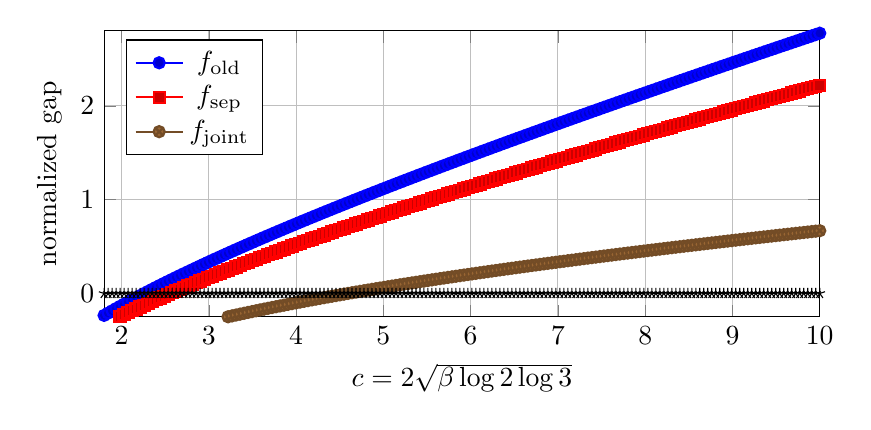
\begin{tikzpicture}
\begin{axis}[
 width=0.88\textwidth,height=0.43\textwidth,
 xlabel={$c=2\sqrt{\beta\log2\log3}$},
 ylabel={normalized gap},
 xmin=1.8,xmax=10,ymin=-0.25,ymax=2.8,
 grid=major,legend pos=north west,
 samples=180,
]
\addplot+[thick,domain=1.8:10] {0.5*ln(x)-1+(11/6-pi/2)*x};
\addlegendentry{$f_{\rm old}$}
\addplot+[thick,domain=1.8:10] {0.5*ln(x)-1+(16/9-pi/2)*x};
\addlegendentry{$f_{\rm sep}$}
\addplot+[thick,domain=1.8:10] {0.5*ln(x)-1+(4/9-pi/8)*x};
\addlegendentry{$f_{\rm joint}$}
\addplot+[black,dashed,domain=1.8:10] {0};
\end{axis}
\end{tikzpicture}
\caption{The three triangular gap functions.  The joint screen crosses zero
at $c=4.5934162\ldots$, corresponding to $\beta=6.9269443\ldots$.}
\label{fig:tri-gaps}
\end{figure}

\section{HCIZ free-energy reconnaissance}
\label{sec:hciz-numerics}

The preceding no-go theorem does not require the exact HCIZ free energy.
Nevertheless, numerical evaluation is useful for measuring how much entropy
is actually present and for calibrating new geometries.

\subsection{A stable determinant formula}

For triangular quantile nodes
\[
 x_i=\sqrt{\frac{i+1/2}{N}},\qquad 0\le i<N,
\]
and scaled spectra $u_i=\sqrt N\,U x_i$,
$v_i=\sqrt N\,V x_i$, put $t=Nc$.  The HCIZ identity becomes
\begin{equation}\label{eq:HCIZ-quantile-formula}
 I_N=G(N+1)t^{-N(N-1)/2}
 \frac{\det(\e^{t x_i x_j})_{0\le i,j<N}}{\DeltaV(x)^2}.
\end{equation}
High precision is essential: the numerator determinant is totally positive
but extremely ill-conditioned in ordinary floating-point arithmetic.

\begin{center}
\resizebox{\textwidth}{!}{%
\begin{tabular}{@{}lrrrrrr@{}}
\toprule
$c$ & $N=8$ & $N=12$ & $N=16$ & $N=20$
 & Jensen $4c/9$ & forward $c/2$\\
\midrule
$2.1972245773$ & $0.9902881602$ & $0.9875417092$ & $0.9863697075$ & $0.9857446579$
 & $0.9765442566$ & $1.0986122887$\\
$2.5603078840$ & $1.1552417262$ & $1.1521074196$ & $1.1507724885$ & $1.1500614614$
 & $1.1379146151$ & $1.2801539420$\\
$4.5934162236$ & $2.0855796790$ & $2.0806140315$ & $2.0785278197$ & $2.0774272195$
 & $2.0415183216$ & $2.2967081118$\\
$9.0687375706$ & $4.1684482612$ & $4.1609010095$ & $4.1578193572$ & $4.1562264719$
 & $4.0305500314$ & $4.5343687853$\\
\bottomrule
\end{tabular}}
\end{center}
All entries in the four middle columns are $N^{-2}\log I_N$ computed from
\eqref{eq:HCIZ-quantile-formula}.  They lie strictly between the Jensen and
forward bounds, as they must.  The table is numerical reconnaissance, not a
proof of convergence or a certified enclosure.

\subsection{An exact variance identity}

\begin{lemma}[Haar trace variance]\label{lem:Haar-variance}
Let $A,B$ be Hermitian $N\times N$ matrices and put
$A_0=A-(\Tr A/N)I$, $B_0=B-(\Tr B/N)I$.  If $U$ is Haar distributed on
$U(N)$, then
\begin{equation}\label{eq:Haar-variance}
 \Var\bigl(\Tr(AUBU^*)\bigr)
 =\frac{\Tr(A_0^2)\Tr(B_0^2)}{N^2-1}.
\end{equation}
\end{lemma}

\begin{proof}
Unitary invariance reduces the covariance tensor of
$UB_0U^*$ to a linear combination of the identity and flip tensors.  The
conditions $\Tr B_0=0$ and
$\E\Tr((UB_0U^*)^2)=\Tr(B_0^2)$ determine the coefficients; contraction with
$A_0\otimes A_0$ gives~\eqref{eq:Haar-variance}.  Equivalently, it follows
immediately from the second-order unitary Weingarten formula
\[
 \E(U_{ij}\overline{U_{kl}}U_{mn}\overline{U_{rs}})
 =\frac{\delta_{ik}\delta_{mr}\delta_{jl}\delta_{ns}
       +\delta_{ir}\delta_{mk}\delta_{js}\delta_{nl}}{N^2-1}
 -\frac{\delta_{ik}\delta_{mr}\delta_{js}\delta_{nl}
       +\delta_{ir}\delta_{mk}\delta_{jl}\delta_{ns}}{N(N^2-1)}.
\]
\end{proof}

For the triangular law, $\Var(X)=1/18$.  Therefore the second Taylor
coefficient of the centered HCIZ logarithm satisfies
\begin{equation}\label{eq:HCIZ-second-coeff}
 \frac1{2N^2}\Var\bigl(\Tr(AUBU^*)\bigr)
 \longrightarrow \frac{c^2}{648}.
\end{equation}
More explicitly, after writing the amplitude as a scalar parameter $\lambda$,
the finite-$N$ identity is
\[
 \frac1{N^2}\log\E\exp\!\bigl(\lambda Z_N\bigr)
 =\lambda\frac{M_N}{N^2}
  +\frac{\lambda^2}{2N^2}\Var(Z_N)+O_N(\lambda^3).
\]
Thus the Jensen floor is not asymptotically exact even infinitesimally: the
first entropy correction is positive and of order $N^2$.

\begin{warningbox}[Interpretation]
The exact variance calculation explains the numerical gap but does not create
a proof route.  In the triangular family the geometric screen is already
positive for every hypothetical exponent left by the inherited results.
Any positive entropy only worsens that obstruction.
\end{warningbox}

\section{A general screen functional and power-cusp geometries}
\label{sec:cusp}

The triangular obstruction is a statement about one limiting spectral shape,
not about all exact-grid determinants.  This section derives the general
screen functional and then constructs a family for which that functional is
negative.  The construction is a genuine advance: it proves that the positive
triangular screen can be escaped.  It is not yet a proof, because the adelic
alignment term can be large.

\subsection{The continuum screen}

For a compactly supported atomless probability measure $\mu$ on $[0,\infty)$,
write $Q_\mu$ for its increasing quantile, $m_\mu$ for its mean, and
\begin{equation}\label{eq:log-energy}
 \mathcal E(\mu)=\iint\log|x-y|\dd\mu(x)\dd\mu(y),
\end{equation}
assuming the logarithmic energy is finite.

\begin{theorem}[Continuum geometric screen]\label{thm:continuum-screen}
Suppose exact-grid spectra satisfy
\[
 \frac{u_i}{\sqrt N}\Longrightarrow\mu,
 \qquad
 \frac{v_i}{\sqrt N}\Longrightarrow\nu,
\]
with convergence strong enough for the logarithmic energies and first
moments to converge.  Then
\begin{equation}\label{eq:screen-functional}
 \frac{S_N}{N^2}\longrightarrow
 \mathscr S(\mu,\nu):=
 \frac12\mathcal E(\mu)+\frac12\mathcal E(\nu)+\frac34
 +m_\mu m_\nu
 -\int_0^1Q_\mu(s)Q_\nu(1-s)\dd s.
\end{equation}
\end{theorem}

\begin{proof}
The two Vandermonde limits and the Barnes asymptotic are exactly those used in
Lemma~\ref{lem:tri-energy}.  The product of empirical means converges to
$m_\mu m_\nu$.  Finally, the rearrangement theorem identifies the reverse
assignment limit with the countermonotone transport integral.  Substitution
in $S_N=V_N+M_N-C_N^-$ proves~\eqref{eq:screen-functional}.
\end{proof}

The theorem turns the geometric part of the determinant problem into a
variational question.  A necessary condition for a termwise-valuation proof
is a pair of realizable spectral measures with $\mathscr S<0$.  This condition
is not sufficient: one must still control $H_N+A_N$.

\subsection{A family of realizable cusps}

Fix an integer $q\ge2$.  In the first-quadrant log-coordinate plane write
\[
 x=t\lambda,
 \qquad y=t(1-\lambda),
\]
so that the Jacobian is $t$.  Define
\begin{equation}\label{eq:Rq}
 \mathcal R_q=
 \left\{0\le t\le1:\
 \left|\lambda-\frac12\right|\le\frac12t^{q-2}\right\}.
\end{equation}
The region is a narrowing cusp around the diagonal $x=y$, and
\begin{equation}\label{eq:Rq-area}
 |\mathcal R_q|=\int_0^1t\,t^{q-2}\dd t=\frac1q.
\end{equation}

For the row lattice, use the physical coordinates
$x=\alpha a/(U_q\sqrt N)$, $y=\gamma b/(U_q\sqrt N)$; for the column lattice
use $x=n/(V_q\sqrt N)$, $y=\beta k/(V_q\sqrt N)$, where
\begin{equation}\label{eq:UqVq}
 U_q=\sqrt{q\alpha\gamma},
 \qquad
 V_q=\sqrt{q\beta},
 \qquad
 c_q=U_qV_q=qz,
 \qquad z=\sqrt{\beta\alpha\gamma}.
\end{equation}
Lattice Riemann sums in dilates of~\eqref{eq:Rq} produce exact lattice subsets up
to $o(N)$ boundary modifications; such modifications do not affect any
$N^2$ limit below.  The radial coordinate has density
\begin{equation}\label{eq:cusp-radial-density}
 \rho_q(t)=q t^{q-1},\qquad 0\le t\le1,
\end{equation}
because the cross-sectional area element is $t^{q-1}\dd t$.

\begin{lemma}[Exact cusp energy and transport]\label{lem:cusp-energy}
Let $T_q$ have density~\eqref{eq:cusp-radial-density}.  Then
\begin{align}
 m_q:=\E T_q&=\frac q{q+1},\label{eq:cusp-mean}\\
 \mathcal E_q:=\E\log|T_q-T_q'|
 &=-H_q-\frac1{2q},\label{eq:cusp-energy}\\
 B_q:=\int_0^1Q_q(s)Q_q(1-s)\dd s
 &=\mathrm B\!\left(1+\frac1q,1+\frac1q\right),\label{eq:cusp-B}
\end{align}
where $H_q=\sum_{j=1}^qj^{-1}$ and $Q_q(s)=s^{1/q}$.
\end{lemma}

\begin{proof}
The mean and quantile are immediate.  For the energy, symmetry and the
substitution $y=xt$ give
\begin{align*}
 \mathcal E_q
 &=2q^2\int_0^1x^{q-1}\int_0^xy^{q-1}\log(x-y)\dd y\dd x\\
 &=2q^2\int_0^1x^{2q-1}\dd x
   \int_0^1t^{q-1}\bigl(\log x+\log(1-t)\bigr)\dd t\\
 &=-\frac1{2q}+q\int_0^1t^{q-1}\log(1-t)\dd t
 =-\frac1{2q}-H_q.
\end{align*}
The last formula follows from the beta integral.
\end{proof}

\begin{theorem}[Power-cusp screen]\label{thm:cusp-screen}
For the cusp families above,
\begin{equation}\label{eq:cusp-screen}
 \boxed{
 \mathscr S_q(z)=
 \frac12\log(qz)+\frac34-H_q-\frac1{2q}
 +qz\left[
 \left(\frac q{q+1}\right)^2
 -\mathrm B\!\left(1+\frac1q,1+\frac1q\right)
 \right].}
\end{equation}
For every fixed $z>0$,
\begin{equation}\label{eq:cusp-screen-asymptotic}
 \mathscr S_q(z)
 =-\frac12\log q+\frac12\log z+\frac34-\gamma_{\!E}+o(1)
 \longrightarrow-\infty.
\end{equation}
Thus realizable exact-grid geometries with a negative joint screen exist for
every hypothetical counterexample.
\end{theorem}

\begin{proof}
Scale the law of $T_q$ by $U_q$ and $V_q$ in
Theorem~\ref{thm:continuum-screen}.  The two energy terms contribute
$\frac12\log(qz)+\mathcal E_q$, the mean term is $qz m_q^2$, and the reverse
transport is $qzB_q$.  This proves~\eqref{eq:cusp-screen}.

Put $\varepsilon=1/q$.  The standard gamma expansion gives
\begin{align*}
 \left(\frac q{q+1}\right)^2
 &=1-2\varepsilon+3\varepsilon^2+O(\varepsilon^3),\\
 \mathrm B(1+\varepsilon,1+\varepsilon)
 &=1-2\varepsilon+\bigl(4-\tfrac{\pi^2}{6}\bigr)\varepsilon^2
   +O(\varepsilon^3).
\end{align*}
Hence their difference is
$(\pi^2/6-1)q^{-2}+O(q^{-3})$.  Together with
$H_q=\log q+\gamma_{\!E}+1/(2q)+O(q^{-2})$, this yields
\eqref{eq:cusp-screen-asymptotic}.
\end{proof}

For the two finite endpoints relevant to the computation, the screen crosses
zero already at $q=9$:
\begin{center}
\begin{tabular}{@{}rrrr@{}}
\toprule
$q$ & $m_q^2-B_q$ & $\mathscr S_q(z_{27})$ & $\mathscr S_q(z_{28})$\\
\midrule
$2$  & $0.0517453627$ & $ 0.5716816488$ & $ 0.5893846472$\\
$4$  & $0.0219751076$ & $ 0.3892297577$ & $ 0.4056355442$\\
$6$  & $0.0118358913$ & $ 0.1903991210$ & $ 0.2053999611$\\
$8$  & $0.0073547992$ & $ 0.0320015476$ & $ 0.0459891876$\\
$9$  & $0.0060106952$ & $-0.0347761982$ & $-0.0211831341$\\
$10$ & $0.0050029689$ & $-0.0949797019$ & $-0.0817250021$\\
$12$ & $0.0036203266$ & $-0.1995903265$ & $-0.1868836047$\\
$16$ & $0.0021453252$ & $-0.3641985599$ & $-0.3522505734$\\
\bottomrule
\end{tabular}
\end{center}
Here $z_b=\sqrt{b\log2\log3}$.  The negative entries show exactly how much
room is available for $H_N+A_N$; they do not assert that either defect is
small.

\subsection{HCIZ entropy in the cusp family}

For quantile nodes
$x_i=((i+1/2)/N)^{1/q}$, formula~\eqref{eq:HCIZ-quantile-formula} remains valid
with $c$ replaced by $c_q=qz$.  At $\beta=28$ and $N=32$, high-precision
reconnaissance gives:
\begin{center}
\begin{tabular}{@{}rrrr@{}}
\toprule
$q$ & $H_N/N^2$ & variance prediction
$\frac12c_q^2\Var(T_q)^2$ & screen $\mathscr S_q(z_{28})$\\
\midrule
$9$  & $0.0662792945$ & $0.0578072909$ & $-0.0211831341$\\
$10$ & $0.0584731296$ & $0.0505667121$ & $-0.0817250021$\\
$12$ & $0.0460717253$ & $0.0394905746$ & $-0.1868836047$\\
$16$ & $0.0299562636$ & $0.0258188672$ & $-0.3522505734$\\
$24$ & $0.0147022573$ & $0.0133947985$ & $-0.5814338175$\\
\bottomrule
\end{tabular}
\end{center}
The variance entry is exact at second order because
\begin{equation}\label{eq:cusp-variance}
 \Var(T_q)=\frac{q}{(q+1)^2(q+2)},
 \qquad
 \frac12c_q^2\Var(T_q)^2
 =\frac{q^4z^2}{2(q+1)^4(q+2)^2}.
\end{equation}
The entropy decreases with $q$ in this experiment, much more slowly than the
screen at first.  For $q\ge10$ the numerical screen has enough room to absorb
the observed HCIZ entropy.  The remaining and more serious issue is the
adelic alignment defect.

\subsection{The separated-support obstruction}
\label{sec:cusp-obstruction}

The inherited arithmetic constraints do not exclude
\begin{equation}\label{eq:separated-support}
 \gcd(M,6)=\gcd(A,6)=\gcd(M,A)=1.
\end{equation}
Under~\eqref{eq:separated-support}, the supports of the four logarithmic
rank-one components are pairwise disjoint.  Primewise minimization therefore
separates exactly.

\begin{theorem}[Cusp failure in the separated-support branch]
\label{thm:cusp-separated}
Assume~\eqref{eq:separated-support}.  For the power-cusp grids,
\begin{equation}\label{eq:cusp-Tsep-limit}
 \frac{T_N}{N^2}=4c_qK_q+o(1),
\end{equation}
where $K_q$ is the countermonotone product of either coordinate marginal in
$\mathcal R_q$.  Moreover
\begin{equation}\label{eq:Kq-limit}
 K_q\longrightarrow\frac29,
 \qquad
 \frac{M_N-T_N}{N^2}
 =qz\left(m_q^2-4K_q\right)+o(1)
 \sim\frac{qz}{9}.
\end{equation}
Consequently
\[
 \frac{V_N+M_N-T_N}{N^2}\longrightarrow+\infty
 \qquad(q\to\infty).
\]
Thus power-cusp concentration cannot yield a universal proof by separate
termwise valuations.
\end{theorem}

\begin{proof}
Under~\eqref{eq:separated-support}, primes dividing $2$, $3$, $M$, and $A$
see respectively the costs $an$, $bn$, $ak$, and $bk$, up to their fixed
logarithmic weights.  Each cost has its own one-dimensional reverse matching,
so equality holds in the componentwise separation.  Symmetry of
$\mathcal R_q$ makes all four normalized minima equal to $c_qK_q$.

Conditioned on the radial variable $T=t$, either coordinate has the exact
representation
\begin{equation}\label{eq:cusp-coordinate}
 X_q=\frac t2+\frac{t^{q-1}}2Z,
 \qquad Z\sim\operatorname{Unif}[-1,1].
\end{equation}
As $q\to\infty$, $T\to1$ in probability and $T^{q-1}$ converges in law to an
independent $S\sim\operatorname{Unif}[0,1]$.  Hence
\[
 X_q\Longrightarrow X_\infty=\frac{1+SZ}{2}.
\]
The limit law is symmetric about $1/2$, has mean $1/2$, and has variance
$\E(S^2)\E(Z^2)/4=1/36$.  For a distribution symmetric about $1/2$, the
countermonotone partner of $X$ is $1-X$, so
\[
 K_q\longrightarrow\E[X_\infty(1-X_\infty)]
 =\frac14-\frac1{36}=\frac29.
\]
Since $m_q\to1$, $m_q^2-4K_q\to1/9$.  The Vandermonde part grows only like
$-\frac12\log q+O(1)$ by~\eqref{eq:cusp-screen-asymptotic}, while the displayed
deficit grows linearly in $q$.
\end{proof}

\begin{warningbox}[What the cusp result does and does not prove]
The family solves the purely geometric variational problem
$\mathscr S<0$.  It also proves that geometry alone is insufficient: a
prime-support pattern still compatible with every inherited theorem makes
$A_N$ large enough to reverse the gain.  A successful determinant family
must couple the prime assignments intrinsically, rather than merely
concentrate the real spectra.
\end{warningbox}

\section{A universal factorial divisor from integer-valued interpolation}
\label{sec:factorial}

The determinant method has so far used only prime factors already present in
the entries.  Integer evaluation matrices also acquire unavoidable
``new-prime'' divisors from finite-difference algebra.  The next theorem is
universal and appears not to have been used in the inherited report.

\begin{definition}
A finite set $\mathcal S\subset\Nzero^2$ is a \emph{coordinate lower set} if
$(n,k)\in\mathcal S$ and $0\le r\le n$, $0\le s\le k$ imply
$(r,s)\in\mathcal S$.  Put
\begin{equation}\label{eq:factorial-product}
 \mathfrak F(\mathcal S)=\prod_{(n,k)\in\mathcal S}n!\,k!.
\end{equation}
\end{definition}

\begin{theorem}[Lower-set factorial divisor]\label{thm:factorial-divisor}
Let $\mathcal S\subset\Nzero^2$ be a lower set of cardinality $N$, and let
$(X_i,Y_i)\in\Z^2$, $1\le i\le N$.  Then
\begin{equation}\label{eq:factorial-divisibility}
 \mathfrak F(\mathcal S)
 \ \bigm|\ 
 \det\bigl(X_i^nY_i^k\bigr)_{1\le i\le N,\ (n,k)\in\mathcal S}.
\end{equation}
\end{theorem}

\begin{proof}
Use the binomial basis
$\binom Xr\binom Ys$.  The Stirling expansion is
\begin{equation}\label{eq:stirling-binomial}
 X^nY^k
 =\sum_{r\le n}\sum_{s\le k}
 \genfrac\{\}{0pt}{}{n}{r}
 \genfrac\{\}{0pt}{}{k}{s}
 r!s!\binom Xr\binom Ys,
\end{equation}
where the braces denote Stirling numbers of the second kind.  Because
$\mathcal S$ is lower, an order extending the coordinate partial order makes
the column-change matrix triangular, with diagonal entries $n!k!$.  The
binomial evaluation matrix has integer entries for every integer $X_i,Y_i$.
Taking determinants in~\eqref{eq:stirling-binomial} proves the divisibility.
\end{proof}

The theorem applies to the exact grid in two ways.  If the row exponent set
$\mathcal R$ is lower, transpose the evaluation matrix and use the integer
points $(2^nM^k,3^nA^k)$.  If the column exponent set $\mathcal C$ is lower,
use the integer points $(2^a3^b,M^aA^b)$.  Thus $D_N$ is divisible by both
$\mathfrak F(\mathcal R)$ and $\mathfrak F(\mathcal C)$, although their full
product need not divide without additional hypotheses.

\subsection{Exact growth on weighted triangles}

Let $\mathcal S_N(w_1,w_2)$ be the first $N$ lattice points in increasing
order of $w_1n+w_2k$, with $w_1,w_2>0$.  This is a lower set, up to an
irrelevant choice among finitely many boundary ties.

\begin{theorem}[Factorial asymptotic]\label{thm:factorial-asymptotic}
As $N\to\infty$,
\begin{equation}\label{eq:factorial-asymptotic}
 \log\mathfrak F(\mathcal S_N(w_1,w_2))
 =\frac{\sqrt2}{6}\frac{w_1+w_2}{\sqrt{w_1w_2}}
 N^{3/2}\log N+O_{w_1,w_2}(N^{3/2}).
\end{equation}
If a fixed finite set of primes is deleted from the prime factorization of
$\mathfrak F$, the leading term is unchanged.
\end{theorem}

\begin{proof}
The threshold $R_N$ satisfies
\[
 N=\frac{R_N^2}{2w_1w_2}+O(R_N),
 \qquad
 R_N=\sqrt{2w_1w_2N}+O(1).
\]
Stirling's formula and a lattice Riemann sum reduce the leading logarithmic
term to one half of $\log N$ times the first coordinate moments:
\begin{align*}
 \sum_{w_1n+w_2k\le R_N}(n+k)
 &=\frac{R_N^3}{6}
 \left(\frac1{w_1^2w_2}+\frac1{w_1w_2^2}\right)+O(N)\\
 &=\frac{\sqrt2}{3}\frac{w_1+w_2}{\sqrt{w_1w_2}}N^{3/2}+O(N).
\end{align*}
Multiplication by $\frac12\log N$ gives~\eqref{eq:factorial-asymptotic}; all
remaining Stirling and boundary terms are $O(N^{3/2})$.

For a fixed prime $p$, Legendre's formula gives
$v_p(n!)=n/(p-1)+O(\log n)$.  Its total logarithmic contribution over the
triangle is therefore $O_p(N^{3/2})$.  Deleting finitely many primes changes
only the error term.
\end{proof}

Let
\[
 \mathcal P_0=\{p:p\mid6MA\}.
\]
All entry primes, and therefore all primes of $Q_N$, lie in $\mathcal P_0$.
Write $\mathfrak F_{\mathcal P_0^c}$ for the part of $\mathfrak F$ supported
outside $\mathcal P_0$.

\begin{corollary}[Universal new-prime excess]\label{cor:new-prime-excess}
If $\mathcal R$ is lower, then
\[
 \Xi_N=\log(D_N/Q_N)
 \ge\log\mathfrak F_{\mathcal P_0^c}(\mathcal R).
\]
If both $\mathcal R$ and $\mathcal C$ are lower, the right side may be
replaced by the larger of the corresponding row and column quantities.  For
the triangular grids,
\begin{align}
 \log\mathfrak F_{\mathcal P_0^c}(\mathcal R_N)
 &=0.483958920105405\ldots\,N^{3/2}\log N+O(N^{3/2}),\label{eq:row-factor-coeff}\\
 \log\mathfrak F_{\mathcal P_0^c}(\mathcal C_N)
 &=\frac{\sqrt2}{6}\frac{1+\beta}{\sqrt\beta}
 N^{3/2}\log N+O_\beta(N^{3/2}).\label{eq:col-factor-coeff}
\end{align}
At $\beta=28$, the second coefficient is
$1.291762669243385\ldots$.
\end{corollary}

\begin{proof}
Theorem~\ref{thm:factorial-divisor} gives the divisibility of $D_N$.  Outside
$\mathcal P_0$ the tropical divisor $Q_N$ has valuation zero, so the same
prime powers divide $D_N/Q_N$.  The constants follow from
Theorem~\ref{thm:factorial-asymptotic} with weights $(\alpha,\gamma)$ and
$(1,\beta)$.
\end{proof}

\begin{warningbox}[A rigorous but subcritical gain]
The factorial divisor is a genuine source of determinant primes not present
in any matrix entry.  Its size is nevertheless
$N^{3/2}\log N=o(N^2)$.  Since every critical geometric and HCIZ term is of
order $N^2$, ordinary integer-valued interpolation cannot repair a positive
leading screen.  A successful arithmetic refinement must create
$N^2$-scale divisibility or cancellation.
\end{warningbox}

\section{Exact signed-progression determinants and the denominator tax}
\label{sec:progression}

Continued fractions suggest choosing exponent vectors along nearly level
lines of the two logarithmic forms.  Signed directions can make both row and
column spacings tiny.  The following family captures that idea exactly and,
crucially, keeps every original exponent nonnegative.

Fix positive integers $p,q,r,s$ and set, for $0\le i,j<N$,
\begin{equation}\label{eq:progression-sets}
 (a_i,b_i)=\bigl(iq,(N-1-i)p\bigr),
 \qquad
 (n_j,k_j)=\bigl(jr,(N-1-j)s\bigr).
\end{equation}
Put
\begin{equation}\label{eq:XYZW}
 X=2^{qr},\qquad Y=3^{pr},\qquad
 Z=M^{qs},\qquad W=A^{ps},
 \qquad P=XW,\quad Q=YZ.
\end{equation}
Then
\begin{equation}\label{eq:progression-eta-product}
 \log\frac PQ
 =(q\alpha-p\gamma)(r-s\beta).
\end{equation}
Thus two independent rational approximations multiply their errors.

\subsection{Complete factorization}

\begin{theorem}[Signed-progression factorization]\label{thm:progression-factor}
For the matrix~\eqref{eq:integer-entry} built from
\eqref{eq:progression-sets},
\begin{equation}\label{eq:progression-factor}
 |D_N|=(PQ)^{\binom N3}
 \prod_{d=1}^{N-1}|P^d-Q^d|^{N-d}.
\end{equation}
The determinant is nonzero because neither factor in
\eqref{eq:progression-eta-product} vanishes.
\end{theorem}

\begin{proof}
A direct expansion of the four exponents gives
\[
 E_{ij}=W^{(N-1)^2}
 \left(\frac ZW\right)^{(N-1)i}
 \left(\frac YW\right)^{(N-1)j}
 \left(\frac PQ\right)^{ij}.
\]
After extracting row and column factors, the remaining matrix is
$(t^{ij})_{0\le i,j<N}$ with $t=P/Q$.  Its Vandermonde determinant is
\begin{equation}\label{eq:geometric-vandermonde}
 \det(t^{ij})
 =t^{\binom N3}\prod_{d=1}^{N-1}(t^d-1)^{N-d}.
\end{equation}
Collecting the powers of $Q$ yields exactly~\eqref{eq:progression-factor}.
The irrationalities $\alpha/\gamma\notin\Q$ and $\beta\notin\Q$ imply
$q\alpha-p\gamma\ne0$ and $r-s\beta\ne0$.
\end{proof}

The monomial factor in~\eqref{eq:progression-factor} is a rational gauge
artifact.  Proposition~\ref{prop:rational-gauge} removes it completely.
Let $g=\gcd(P,Q)$ and write
\[
 \widehat P=P/g,
 \qquad
 \widehat Q=Q/g,
 \qquad
 \gcd(\widehat P,\widehat Q)=1.
\]

\begin{theorem}[Exact invariant local quotient]\label{thm:progression-quotient}
Let $Q_N^{\rm trop}$ be the termwise tropical divisor of the original integer
matrix.  Then
\begin{equation}\label{eq:progression-quotient}
 \boxed{
 \frac{|D_N|}{Q_N^{\rm trop}}
 =\prod_{d=1}^{N-1}
 |\widehat P^{\,d}-\widehat Q^{\,d}|^{N-d}.}
\end{equation}
In particular, every quantity on the right is an ordinary positive integer;
all row, column, and common-gcd heights have already been paid.
\end{theorem}

\begin{proof}
By rational gauge invariance it suffices to calculate the quotient for
$(t^{ij})$ with $t=\widehat P/\widehat Q$.  If
$v_\ell(t)>0$, the reverse assignment minimizes
$v_\ell(t)\sum_i i\sigma(i)$ and its value is
$\binom N3v_\ell(\widehat P)$.  If $v_\ell(t)<0$, the forward assignment
maximizes the sum, giving
$-\bigl(\sum_{i=0}^{N-1}i^2\bigr)v_\ell(\widehat Q)$.  Formula
\eqref{eq:geometric-vandermonde} shows that these are exactly the valuations
of its pure numerator and denominator powers.  Since
$\widehat P^d-\widehat Q^d$ is coprime to both $\widehat P$ and
$\widehat Q$, division by the local tropical factor leaves precisely the
product in~\eqref{eq:progression-quotient}.
\end{proof}

\subsection{Near-collision expansion}

Set
\begin{equation}\label{eq:eta-B}
 \eta=\left|\log\frac{\widehat P}{\widehat Q}\right|>0,
 \qquad B=\min(\widehat P,\widehat Q).
\end{equation}
For $t\ge0$, define
$\rho(t)=\log((\e^t-1)/t)$, with $\rho(0)=0$.  The elementary bounds
$1\le(\e^t-1)/t\le\e^t$ give
\begin{equation}\label{eq:rho-bound}
 0\le\rho(t)\le t.
\end{equation}

\begin{theorem}[Exact denominator-tax expansion]\label{thm:denominator-tax}
The invariant quotient in~\eqref{eq:progression-quotient} satisfies
\begin{equation}\label{eq:denominator-tax}
 \log\frac{|D_N|}{Q_N^{\rm trop}}
 =\binom{N+1}{3}\log B
  +\binom N2\log\eta
  +\log G(N+1)+R_N,
\end{equation}
where
\begin{equation}\label{eq:R-bound}
 0\le R_N\le\binom{N+1}{3}\eta.
\end{equation}
Moreover the integer gap gives
\begin{equation}\label{eq:integer-gap}
 1\le|\widehat P-\widehat Q|
 =B(\e^\eta-1)\le B\eta\e^\eta,
 \qquad
 \log B+\log\eta\ge-\eta.
\end{equation}
Consequently, for $0<\eta\le1$,
\begin{equation}\label{eq:denominator-tax-lower}
 \log\frac{|D_N|}{Q_N^{\rm trop}}
 \ge\binom N3\log\frac1\eta
   -\binom{N+1}{3}\eta+\log G(N+1).
\end{equation}
\end{theorem}

\begin{proof}
For each $d$,
\[
 |\widehat P^d-\widehat Q^d|
 =B^d(\e^{d\eta}-1)
 =B^d d\eta\,\e^{\rho(d\eta)}.
\]
Substitute this identity in~\eqref{eq:progression-quotient}.  The three sums
are
\[
 \sum_{d=1}^{N-1}d(N-d)=\binom{N+1}{3},\quad
 \sum_{d=1}^{N-1}(N-d)=\binom N2,
\]
and
$\sum_{d=1}^{N-1}(N-d)\log d=\log G(N+1)$.  Bound the remainder with
\eqref{eq:rho-bound}.  The gap~\eqref{eq:integer-gap} follows because two
distinct integers differ by at least one.  Finally
$\log B\ge-\log\eta-\eta$ in~\eqref{eq:denominator-tax}, and
$\binom{N+1}{3}-\binom N2=\binom N3$.
\end{proof}

\begin{corollary}[Why double continued fractions do not close the proof]
\label{cor:double-cf-no-go}
Choose $p/q$ among convergents to $\alpha/\gamma$ and $r/s$ among convergents
to $\beta$.  Then
\[
 \eta=|(q\alpha-p\gamma)(r-s\beta)|=O((qs)^{-1}).
\]
Even after every rational gauge and common factor is removed,
\eqref{eq:denominator-tax-lower} forces a positive cubic-in-$N$ denominator
cost of size at least
\[
 \binom N3\log(qs)-O(N^3/(qs))+\log G(N+1).
\]
Thus the quadratic gain $\binom N2\log\eta$ from the apparently tiny spacing
is overpaid by the integer denominator needed to realize that spacing.
\end{corollary}

The factorization also exposes all non-tropical valuations:
\begin{equation}\label{eq:progression-valuation}
 v_\ell(D_N)=\binom N3\bigl(v_\ell(P)+v_\ell(Q)\bigr)
 +\sum_{d=1}^{N-1}(N-d)v_\ell(P^d-Q^d).
\end{equation}
For primes satisfying the standard hypotheses, the lifting-the-exponent
lemma evaluates the last term explicitly.  Hence any future use of this
family must exploit structured cancellation inside cyclotomic factors
$\widehat P^d-\widehat Q^d$; there is no unaccounted archimedean smallness left.

\section{The fewnomial bridge to the Matrix Coefficient Conjecture}
\label{sec:fewnomial}

The rank-one logarithm matrix~\eqref{eq:Lbeta} is exactly the $2\times2$ case
of the Matrix Coefficient Conjecture.  Dasgupta and Kakde prove that their
support condition $(m')$ implies the desired rational coefficient vanishing,
but the implication from singularity $(w)$ to $(m')$ remains open
\cite{DasguptaKakde}.  The integer-output hypothesis gives a particularly
clean version of their zero-count mechanism.

Consider the transposed integer orbit
\begin{equation}\label{eq:fewnomial-grid}
 \mathcal X_L=
 \left\{\bigl(2^m3^n,M^mA^n\bigr):0\le m,n<L\right\}
 \subset\N^2.
\end{equation}
Every point lies on the transcendental power curve $Y=X^\beta$, and all
$L^2$ points are distinct.

\begin{theorem}[Exact support lower bound]\label{thm:support-lower}
Assume a counterexample $\beta$ exists.  Let
\[
 P(X,Y)=\sum_{(a,b)\in\mathcal S}c_{a,b}X^aY^b
 \in\R[X,Y]
\]
be nonzero, with every displayed coefficient nonzero.  If $P$ vanishes at all
points of $\mathcal X_L$, then
\begin{equation}\label{eq:support-lower}
 |\mathcal S|\ge L^2+1.
\end{equation}
In particular, vanishing on $\mathcal X_{2N}$ requires at least
$4N^2+1$ monomials.
\end{theorem}

\begin{proof}
On the curve $Y=X^\beta$, put $X=\e^z$.  The restriction becomes
\begin{equation}\label{eq:exp-polynomial}
 P(\e^z,\e^{\beta z})
 =\sum_{(a,b)\in\mathcal S}c_{a,b}\e^{(a+b\beta)z}.
\end{equation}
The exponents $a+b\beta$ are distinct because $\beta$ is irrational, so the
right side is a nonzero exponential polynomial with
$K=|\mathcal S|$ terms.  Exponentials with distinct real exponents form a
strict Chebyshev system and a nonzero $K$-term combination has at most
$K-1$ distinct real zeros.  The values
$z=m\alpha+n\gamma$, $0\le m,n<L$, are distinct because
$\alpha/\gamma\notin\Q$.  Hence $K-1\ge L^2$.
\end{proof}

\begin{corollary}[A concrete integer auxiliary-polynomial criterion]
\label{cor:small-value-criterion}
The Alaoglu--Erd\H{o}s conjecture would follow if, under the assumption of a
counterexample and for some $N$, one could construct a nonzero polynomial
$P\in\Z[X,Y]$ with at most $4N^2$ monomials such that
\begin{equation}\label{eq:small-values}
 |P(2^m3^n,M^mA^n)|<1
 \qquad(0\le m,n<2N).
\end{equation}
The stronger Dasgupta--Kakde support target $|\supp P|<N^2$ is more than
sufficient.
\end{corollary}

\begin{proof}
Every value in~\eqref{eq:small-values} is an integer, hence is zero.  This
contradicts Theorem~\ref{thm:support-lower}.
\end{proof}

This criterion isolates the analytic heart of the problem.  The zero estimate
is elementary and sharp enough; the missing step is to manufacture a sparse
integer polynomial whose archimedean values are all below one.  Naive products
that vanish for algebraic reasons have coefficient heights too large, while
Siegel-lemma constructions with small support do not automatically produce
uniform small values on the exponentially large grid.  This is the same
coefficient-height obstruction emphasized in the modern Matrix Coefficient
program.

\begin{researchbox}[A potentially useful reformulation]
Instead of asking first for exact vanishing, seek a support set
$\mathcal S_N$ with $|\mathcal S_N|<N^2$ and integer coefficients $c_w$ for
which the normalized exponential sum
\[
 F_N(z)=\sum_{w=(a,b)\in\mathcal S_N}c_w\e^{(a+b\beta)z}
\]
has a product-formula estimate
\[
 \log|F_N(m\alpha+n\gamma)|_\infty
 +\sum_p\log|F_N(m\alpha+n\gamma)|_p<0
\]
after clearing a common denominator, uniformly on $0\le m,n<2N$.
Integrality would then force every value to vanish.  The determinant
factorizations of Sections~\ref{sec:factorial} and~\ref{sec:progression}
provide exact local factors that could be built into such a normalization.
\end{researchbox}

\section{Audit of additional proof routes}
\label{sec:audit}

The supplied report explored many classical and computational directions.
The new calculations above allow several of them to be classified more
sharply.

\begingroup
\small
\setlength{\tabcolsep}{4pt}
\renewcommand{\arraystretch}{1.06}
\begin{longtable}{@{}>{\raggedright\arraybackslash}p{0.19\textwidth}
>{\raggedright\arraybackslash}p{0.31\textwidth}
>{\raggedright\arraybackslash}p{0.44\textwidth}@{}}
\toprule
Route & What it controls & Precise obstruction in the two-base problem\\
\midrule
\endfirsthead
\multicolumn{3}{c}{Audit of proof routes (continued)}\\
\toprule
Route & What it controls & Precise obstruction in the two-base problem\\
\midrule
\endhead
\midrule
\multicolumn{3}{r}{continued on next page}\\
\endfoot
\bottomrule
\endlastfoot
Baker--Matveev linear forms
& Quantitative lower bounds for a \emph{nonzero} linear form in logarithms of
algebraic numbers
& A counterexample gives the exact bilinear zero
$\log M\log3-\log A\log2=0$.  Turning it into a fixed nonzero linear form
loses the rank-two information.\\

Four Exponentials / Matrix Coefficient
& Exactly the rational rank of the logarithm matrix
& This would settle the conjecture, but the relevant $2\times2$ statement is
itself the open Four Exponentials case.  The sparse auxiliary-polynomial
implication $(w)\Rightarrow(m')$ remains unknown.\\

Pure HCIZ asymptotics
& The archimedean determinant free energy
& For triangular grids, even the Jensen floor plus perfect joint tropical
transport is positive beyond $\beta=6.9269\ldots$; exact HCIZ evaluation alone
cannot help.\\

Componentwise $p$-adic transport
& Prime divisors inherited from individual entry factors
& Primewise minimizing permutations can be incompatible.  The resulting
alignment defect $A_N$ is nonnegative and is linear in the cusp parameter in
an admissible separated-support branch.\\

Continued fractions
& Very small projected row and column spacings
& The invariant quotient formula~\eqref{eq:progression-quotient} shows that
integer denominators overpay the small spacing at cubic order.\\

Congruence collisions / finite differences
& New divisibility from repeated residue classes and integer-valued bases
& The universal factorial gain is only $N^{3/2}\log N$, below the critical
$N^2$ scale.  Fixed-modulus refinements have the same limitation.\\

Confluent determinants and jets
& Replace close nodes by high multiplicity at one node
& Derivatives of $\e^{uv}$ introduce powers of $u$ and $v$, hence logarithms;
the entries cease to be integers and the decisive product-formula gain is
lost unless denominators are controlled adelically.\\

A third independent base
& Six Exponentials supplies one transcendental value among a $2\times3$
array
& If $2^x,3^x,5^x$ were all algebraic and $x\notin\Q$, Six Exponentials would
contradict the $\Q$-independence of $\log2,\log3,\log5$.  The difficulty is
intrinsically the critical two-base case.\\
\bottomrule
\end{longtable}
\addtocounter{table}{-1}
\endgroup

\subsection{Why a fixed finite computation cannot be the final proof}

The finite verifier in Section~\ref{sec:finite} excludes a very large compact
range, but a hypothetical primitive exponent has no known unconditional
upper bound.  The inherited monoid theorem creates infinitely many solutions
from one primitive $\beta$, yet their integer first outputs grow as
$2^nM^k$ and do not force a second primitive generator in a bounded interval.
Consequently computation is valuable for raising the floor and testing
constants, but a proof still needs a scale-free argument.

\subsection{Why the new no-go theorems are useful}

Negative results at the level of methods are not merely postmortems.  They
remove several tempting but insufficient tasks:
\begin{enumerate}[leftmargin=2.2em]
\item no amount of precision in the triangular HCIZ limit can bridge the
joint screen gap;
\item no pair of continued fractions can make the exact progression quotient
small without paying its denominator;
\item no ordinary binomial-basis divisibility argument can generate a leading
$N^2$ term;
\item no cusp geometry can be universal unless it also enforces coupling of
the four prime assignments.
\end{enumerate}
The remaining work is therefore much more focused than at the start of the
continuation.

\section{Directed-rounding finite exclusion}
\label{sec:finite}

This section extends the inherited finite computation while preserving a
strict trust boundary.  The mathematical reduction and the interpretation of
a successful interval test are paper proofs.  Exhausting hundreds of millions
of inputs is a software certificate: it depends on the C compiler, MPFR, the
runtime, and the recorded logs, and has not been replayed by the Lean kernel.

\subsection{Reduction to consecutive-integer separation}

Put
\begin{equation}\label{eq:theta}
 \vartheta=\frac{\log3}{\log2}.
\end{equation}
If $m=2^x\in\N$, then
\begin{equation}\label{eq:mtheta}
 3^x=m^\vartheta.
\end{equation}
The input $m$ is a power of two exactly when $x$ is an integer.  Therefore a
nonintegral counterexample with $2^L\le m<2^{L+1}$ would be a non-power of two
for which $m^\vartheta$ is an integer.

\begin{lemma}[Directed logarithmic certificate]\label{lem:directed-cert}
Let $m,n\in\N$.  If directed-rounding interval arithmetic proves
\begin{equation}\label{eq:directed-ineq}
 \log m\,\log3>\log n\,\log2,
 \qquad
 \log(n+1)\,\log2>\log m\,\log3,
\end{equation}
then
\[
 n<m^\vartheta<n+1,
\]
so $m^\vartheta\notin\Z$.
\end{lemma}

\begin{proof}
All logarithms are positive.  Divide~\eqref{eq:directed-ineq} by
$\log2$ and exponentiate.
\end{proof}

The verifier first obtains a long-double locator
$\lfloor\exp(\vartheta\log m)\rfloor$, but correctness does not depend on that
approximation.  It tests nearby candidates and counts an input as certified
only when the two MPFR inequalities~\eqref{eq:directed-ineq} are both strict.
Thus an inaccurate locator could cause a reported \emph{failure}, never a
false success.

\subsection{Implementation and reproducibility manifest}

The literal verifier is reproduced in Appendix~\ref{app:C-source}.  Its
SHA-256 digest is
\begin{center}
\sha{f888c0d89be9366f01e2d26f339dcbe446556d39d4c5dbcf8f579ec0d0052e1d}.
\end{center}
The run environment was Linux x86-64, GCC~14.2.0, MPFR~4.2.2 linked against
GMP, and five OpenMP threads on an Intel Xeon Platinum 8573C.  Every
transcendental operation and every product entering the certificate used
outward MPFR rounding at $192$ bits.  The range was split into chunks of width
$2^{22}$; Appendix~\ref{app:scan-manifest} lists every chunk.

The new range $[2^{27},2^{28})$ was scanned twice from the exact source.  Both
full scans had zero failures and identical checked counts, extremal margins,
and extremal pairs; their logs differ only in timing data.  The log digests
are
\begin{center}
\sha{d8f782795864b6d6c4ec0a33fdbdbbb57ea46a8dd92fc20690f1ea5ab8ef1519},\\
\sha{a234067d7718c4ec638bb5d4a64ca3178159d118d69d70904654b6bd9749d4df}.
\end{center}

\subsection{Completed dyadic ranges}

\begin{center}
\begin{tabular}{@{}lrrrrl@{}}
\toprule
range & chunks & nonpowers checked & failures & precision & provenance\\
\midrule
$1\le m<2^{27}$ & --- & --- & $0$ & MPFR & inherited scans\\
$2^{27}\le m<2^{28}$ & $32$ & $134{,}217{,}727$ & $0$ & $192$ bits & two full runs\\
$2^{28}\le m<2^{29}$ & $64$ & $268{,}435{,}455$ & $0$ & $192$ bits & full run\\
\bottomrule
\end{tabular}
\end{center}
The canonical $[2^{28},2^{29})$ log has SHA-256 digest
\begin{center}
\sha{b8822a77f9a46ad69a8d52849a80aca3526a63de3f76816e3cad6275d9cf2427}.
\end{center}

For $[2^{27},2^{28})$, the summed CPU-wall measurements printed by the
$32$ chunks were $716.927669$ seconds.  The smallest directed lower margin was
\begin{equation}\label{eq:scan28-lower}
 1.9529773015500319\times10^{-22}
 \quad\text{at}\quad
 (m,n)=(233{,}957{,}087,18{,}397{,}848{,}948{,}879),
\end{equation}
and the smallest directed upper margin was
\begin{equation}\label{eq:scan28-upper}
 5.4449255726026935\times10^{-22}
 \quad\text{at}\quad
 (m,n)=(183{,}569{,}533,12{,}526{,}047{,}934{,}207).
\end{equation}
At high precision, the corresponding ordinary gaps are
\begin{align}
 m^\vartheta-n
 &=5.183687159411222194864071179\ldots\times10^{-9},
 \label{eq:scan28-actual-lower}\\
 n+1-m^\vartheta
 &=9.839670510600579115276881649\ldots\times10^{-9}.
 \label{eq:scan28-actual-upper}
\end{align}
Both extremal inputs were independently replayed at $320$ and $512$ bits,
with the same nearest integer and strictly positive directed margins.

For $[2^{28},2^{29})$, the aggregate results were
\begin{align}
 \text{summed chunk time}&=1468.193778\ \text{seconds},\\
 \min\text{ lower margin}&=4.9141462461940518\times10^{-24},\notag\\[-0.25em]
 &\quad\text{at }(m,n)=(388{,}909{,}543,41{,}170{,}668{,}399{,}174),\label{eq:scan29-lower}\\
 \min\text{ upper margin}&=5.2103670350428438\times10^{-23},\notag\\[-0.25em]
 &\quad\text{at }(m,n)=(501{,}373{,}708,61{,}578{,}600{,}753{,}798).\label{eq:scan29-upper}
\end{align}
High-precision reevaluation gives
\begin{align}
 m^\vartheta-n&=2.918841643468300876710355534\ldots\times10^{-10},\label{eq:scan29-actual-lower}\\
 n+1-m^\vartheta&=4.628845365460026803507495027\ldots\times10^{-9}.\label{eq:scan29-actual-upper}
\end{align}
The two extremal inputs were replayed at $320$ and $512$ bits with unchanged
nearest integers and positive directed margins.  The concatenated replay records have SHA-256 digest
\begin{center}
\sha{afc53d5d5c20ca7f946310ae3dc1f8176f6c5af31eb175c9ff32326e4813919d}.
\end{center}

\begin{theorem}[Software-certified exclusion through $2^{29}$]
\label{thm:finite29}
At the stated software-trust level,
\begin{equation}\label{eq:finite29-statement}
 1\le m<2^{29},\quad m^\vartheta\in\N
 \quad\Longrightarrow\quad
 m\text{ is a power of two}.
\end{equation}
Consequently every nonintegral $x$ satisfying $2^x,3^x\in\Z$ obeys
\begin{equation}\label{eq:x-gt-29}
 \boxed{x>29.}
\end{equation}
\end{theorem}

\begin{proof}
The inherited scans cover $m<2^{27}$, and the two completed new dyadic scans
cover $2^{27}\le m<2^{29}$.  Every non-power input has a strict consecutive-
integer certificate from Lemma~\ref{lem:directed-cert}.  If $m=2^x<2^{29}$
came from a nonintegral solution, then~\eqref{eq:mtheta} would make
$m^\vartheta=3^x$ an integer at a non-power input, a contradiction.  The
endpoint $m=2^{29}$ corresponds to the integral exponent $29$, so a
nonintegral solution must satisfy $m>2^{29}$ and $x>29$.
\end{proof}

\begin{warningbox}[Trust boundary]
Theorem~\ref{thm:finite29} is not a theorem of Lean or of MPFR as a formal
logic.  It is a reproducible exhaustive computation whose source, hashes,
chunk records, precision, and extreme cases are disclosed.  The inherited
kernel-checked floor remains $\beta\ge12$ until a formal interval checker
replays the certificates.
\end{warningbox}

\section{Three precise routes that would finish the conjecture}
\label{sec:proof-program}

The continuation narrows the remaining problem to three mathematically
explicit targets.  They are not vague invitations to ``improve the bounds'':
each is a sufficient theorem with a quantified threshold.

\subsection{Route A: a negative screen with controlled defects}

\begin{proposition}[Determinant completion criterion]\label{prop:det-completion}
Assume a counterexample and suppose there is a sequence of exact-grid
matrices for which, for some $\varepsilon>0$,
\begin{equation}\label{eq:det-completion}
 S_N\le-\varepsilon N^2,
 \qquad
 H_N+A_N=o(N^2).
\end{equation}
Then the Alaoglu--Erd\H{o}s conjecture follows.
More generally it is enough that
$\limsup_N(H_N+A_N)/N^2<\varepsilon$.
\end{proposition}

\begin{proof}
The exact identity
$\Xi_N=S_N+H_N+A_N$ would give $\Xi_N<0$ for all sufficiently large $N$,
contradicting the positive integrality of $D_N/Q_N$.
\end{proof}

The power cusps provide $S_N/N^2<0$ with arbitrarily large magnitude, but
Theorem~\ref{thm:cusp-separated} shows that $A_N$ need not be small.  The
next design problem is therefore not another radial concentration.  It is to
build exponent sets for which every prime cost is forced to use nearly the
same reverse matching.  Promising mechanisms include:
\begin{enumerate}[leftmargin=2.2em]
\item arithmetic coupling of row coordinates, so that $a$ and $b$ are not
      independently reorderable;
\item a multiscale geometry in which any permutation improving one prime
      incurs a larger loss at another prime;
\item an averaging over several determinant blocks whose alignment defects
      cancel or telescope while their negative screens add.
\end{enumerate}
A theorem of the form
$A_N\le C\,H_N+o(N^2)$ with a uniform $C$ would already make the numerical
cusp data actionable for sufficiently large $q$.

\subsection{Route B: an analytic fewnomial}

By Corollary~\ref{cor:small-value-criterion}, it is enough to derive from the
rank-one logarithm relation a sparse integer polynomial with uniformly small
values on $\mathcal X_{2N}$.  A concrete target is:

\begin{problem}[Integer $(w)\Rightarrow(m')$ target]\label{prob:fewnomial-target}
For every sufficiently large $N$, construct under the counterexample
hypothesis a nonzero $P_N\in\Z[X,Y]$ such that
\begin{equation}\label{eq:fewnomial-target}
 |\supp P_N|<N^2,
 \qquad
 \max_{0\le m,n<2N}
 |P_N(2^m3^n,M^mA^n)|<1.
\end{equation}
\end{problem}

The second inequality forces exact vanishing, and
Theorem~\ref{thm:support-lower} then gives an immediate contradiction.  The
advantage over the general Matrix Coefficient setting is that the evaluation
points and coefficients can both be integral.  The disadvantage is that
integrality leaves no room for a merely good approximation: the product
formula must beat the coefficient height at every point simultaneously.

A potentially creative hybrid is to use a determinant cofactor vector as the
coefficient vector of $P_N$.  Sections~\ref{sec:factorial} and
\ref{sec:progression} then provide exact common divisors of the cofactors.
If those divisors reduce the primitive coefficient height by an
$\exp(cN^2)$ factor, the remaining archimedean interpolation error could cross
below one.  The universal factorial divisor alone is too small, but a
cyclotomic or many-prime refinement might reach the critical scale.

\subsection{Route C: non-tropical valuation at quadratic scale}

Termwise tropical divisibility uses only the smallest valuation among
Leibniz terms.  Determinants can have much larger valuation because many
minimum terms cancel modulo powers of a prime.  Let $R_N$ be any explicitly
proved divisor of $D_N$.

\begin{proposition}[Quadratic divisor criterion]\label{prop:quadratic-divisor}
If, for some exact-grid family,
\begin{equation}\label{eq:quadratic-divisor}
 \log R_N>V_N+C_N^++o(N^2),
\end{equation}
then the conjecture follows.
The same conclusion holds with $C_N^+$ replaced by any rigorous upper bound
for $\log I_N$.
\end{proposition}

\begin{proof}
The HCIZ identity and $\log I_N\le C_N^+$ give
$\log D_N\le V_N+C_N^+$.  A positive integer cannot be divisible by an
integer larger than itself.
\end{proof}

Theorem~\ref{thm:factorial-asymptotic} supplies only
$\log R_N\asymp N^{3/2}\log N$.  To reach~\eqref{eq:quadratic-divisor}, one
needs cancellation repeated across a positive proportion of the tropical
layers.  Formula~\eqref{eq:progression-valuation} suggests studying the
cyclotomic decomposition
\[
 \widehat P^d-\widehat Q^d
 =\prod_{e\mid d}\Phi_e(\widehat P,\widehat Q)
\]
together with weighted multiplicities $N-d$.  A theorem forcing many small
orders modulo many primes could create the missing $N^2$ contribution, but it
must be uniform in the unknown integers $M,A$.

\subsection{Formalization roadmap}

The paper-level results most suitable for kernel checking are:
\begin{enumerate}[leftmargin=2.2em]
\item the algebraic factorization
Theorems~\ref{thm:progression-factor} and~\ref{thm:progression-quotient};
\item the binomial-basis divisor Theorem~\ref{thm:factorial-divisor};
\item the support lower bound Theorem~\ref{thm:support-lower};
\item a small reflective checker for each MPFR certificate, replacing trust
      in the exhaustive C loop by a list of verified rational intervals.
\end{enumerate}
The continuum asymptotics and HCIZ analysis are less urgent to formalize
until an arithmetic alignment theorem makes them part of a closing argument.

\section{Conclusion}
\label{sec:conclusion}

The Alaoglu--Erd\H{o}s conjecture remains unproved, but the continuation
changes the shape of the search in several substantive ways.

First, every exact-grid determinant now has an exact accounting identity:
\[
 \log(D_N/Q_N)=S_N+H_N+A_N.
\]
This prevents archimedean geometry, random-matrix entropy, and incompatible
prime assignments from being conflated.  Second, the inherited triangular
family is decisively closed as a route: its best possible joint screen is
positive far below the range already excluded.  Third, power cusps prove that
negative screens are realizable, while the separated-support theorem exposes
the new arithmetic obstacle they create.  Fourth, the exact progression
quotient proves that double continued fractions do not supply free smallness;
the integer denominator is visible term by term.  Fifth, the lower-set
factorial theorem identifies a universal source of new determinant primes and
shows quantitatively why it is still subcritical.  Sixth, the integer orbit
turns the Dasgupta--Kakde fewnomial strategy into the explicit small-value
criterion~\eqref{eq:fewnomial-target}.  Finally, the directed-rounding scan
raises the software-certified floor to $x>29$.

The most promising synthesis is no longer ``one more determinant estimate.''
It is a construction that couples real transport to prime transport: either a
negative-screen family with forced adelic alignment, or a sparse auxiliary
polynomial whose coefficients inherit an $N^2$-scale determinant divisor.
Both formulations attack the precise rank-two obstruction rather than a
surrogate.  They also provide clear falsification tests for future ideas:
compute the screen, expose the denominator gauge, and account for every prime
assignment before investing in a large asymptotic calculation.

\begin{outcomebox}
The requested conjectural proof has not been completed.  The strongest new
unconditional conclusions are the exact determinant decompositions,
no-go theorems, support and divisibility results proved above.  The strongest
new finite conclusion is the reproducible software certificate $x>29$.
The report deliberately leaves the final theorem labelled open rather than
turning a numerical or conjectural step into a false proof.
\end{outcomebox}

\appendix

\section{Constants and elementary integrals}
\label{app:constants}

For reference, the constants used repeatedly in the report are
\begin{align*}
 \alpha&=\log2=0.6931471805599453094\ldots,\\
 \gamma&=\log3=1.0986122886681096914\ldots,\\
 J&=\frac\pi8-\frac13=0.0593657483653908215\ldots,\\
 \delta_{\rm old}&=\frac{11}{6}-\frac\pi2
 =0.2625370065384367141\ldots,\\
 \delta_{\rm sep}&=\frac{16}{9}-\frac\pi2
 =0.2069814509828811585\ldots,\\
 \delta_{\rm joint}&=\frac49-\frac\pi8
 =0.0517453627457202896\ldots.
\end{align*}
The beta integrals are
\begin{align*}
 \int_0^1\sqrt{s(1-s)}\dd s
 &=\mathrm B(3/2,3/2)=\frac\pi8,\\
 \int_0^1(1-\sqrt{1-s})(1-\sqrt s)\dd s
 &=\frac\pi8-\frac13,\\
 \int_0^1[s(1-s)]^{1/q}\dd s
 &=\mathrm B(1+1/q,1+1/q).
\end{align*}
The combinatorial sums used in the progression determinant are
\begin{align*}
 \sum_{i=0}^{N-1}i(N-1-i)&=\binom N3,\\
 \sum_{d=1}^{N-1}d(N-d)&=\binom{N+1}{3},\\
 \sum_{d=1}^{N-1}(N-d)&=\binom N2,\\
 \prod_{d=1}^{N-1}d^{N-d}&=G(N+1).
\end{align*}

\section{High-precision HCIZ reconnaissance code}
\label{app:HCIZ-code}

The following minimal Python/mpmath program evaluates the quantile
formula~\eqref{eq:HCIZ-quantile-formula}.  For large $q$ and $N$, hundreds or
thousands of decimal digits are required because the totally positive
exponential matrix is extremely ill-conditioned.

\begin{lstlisting}[language=Python]
import mpmath as mp


def hciz_log_over_n2(N: int, c, q: int = 2, dps: int = 200):
    """Return (log I_N)/N^2 and the centered entropy H_N/N^2.

    q=2 gives the triangular radial law; general q gives density q*t^(q-1).
    The midpoint quantiles are used.
    """
    mp.mp.dps = dps
    c = mp.mpf(c)
    x = [((mp.mpf(i) + mp.mpf("0.5")) / N) ** (mp.mpf(1) / q)
         for i in range(N)]
    t = N * c
    A = mp.matrix([[mp.exp(t * x[i] * x[j]) for j in range(N)]
                   for i in range(N)])
    det_A = mp.det(A)
    if det_A <= 0:
        raise ArithmeticError("increase dps: determinant was not resolved")

    log_G = sum(mp.log(mp.factorial(j)) for j in range(1, N))
    log_delta = sum(mp.log(x[j] - x[i])
                    for i in range(N) for j in range(i + 1, N))
    pairs = N * (N - 1) // 2
    log_I = log_G - pairs * mp.log(t) + mp.log(det_A) - 2 * log_delta
    mean = sum(x) / N
    entropy = log_I / N**2 - c * mean**2
    return log_I / N**2, entropy


if __name__ == "__main__":
    alpha, gamma = mp.log(2), mp.log(3)
    beta = mp.mpf(28)
    z = mp.sqrt(beta * alpha * gamma)
    for q in (9, 10, 12, 16, 24):
        value, entropy = hciz_log_over_n2(32, q * z, q=q, dps=1600)
        print(q, mp.nstr(value, 20), mp.nstr(entropy, 20))
\end{lstlisting}

\section{Full directed-rounding chunk manifest}
\label{app:scan-manifest}

The following table records every newly executed chunk.  The endpoints are
half-open.  ``Lower'' is the smallest certified value of
$\log m\log3-\log n\log2$ in the chunk; ``upper'' is the smallest certified
value of $\log(n+1)\log2-\log m\log3$.

\begin{landscape}
\pagestyle{empty}
\begingroup
\tiny
\setlength{\tabcolsep}{4pt}
\renewcommand{\arraystretch}{1.02}
\begin{longtable}{@{}r r r r l l r@{}}
\caption{Canonical manifest of all newly executed directed-rounding chunks.  Every row used MPFR 4.2.2 at 192 bits with five OpenMP threads.}\label{tab:scan-manifest}\\
\toprule
chunk & half-open $m$-range & checked & failures & minimum lower margin & minimum upper margin & seconds\\
\midrule
\endfirsthead
\multicolumn{7}{c}{\tablename\ \thetable\ (continued)}\\
\toprule
chunk & half-open $m$-range & checked & failures & minimum lower margin & minimum upper margin & seconds\\
\midrule
\endhead
\midrule
\multicolumn{7}{r}{continued on next page}\\
\endfoot
\bottomrule
\endlastfoot
\multicolumn{7}{@{}l}{\textbf{Dyadic block $2^{27}\le m<2^{28}$}: 32 chunks, 134,217,727 nonpowers, zero failures.}\\
\addlinespace[2pt]
1 & $[134,217,728,138,412,032)$ & $4,194,303$ & 0 & \texttt{4.2836769792074091e-20} & \texttt{3.3891031242020454e-20} & 21.573743\\
2 & $[138,412,032,142,606,336)$ & $4,194,304$ & 0 & \texttt{2.814750234252554e-20} & \texttt{2.8468076218901581e-21} & 22.158163\\
3 & $[142,606,336,146,800,640)$ & $4,194,304$ & 0 & \texttt{1.0607294660531761e-20} & \texttt{6.2725924488237467e-22} & 22.023830\\
4 & $[146,800,640,150,994,944)$ & $4,194,304$ & 0 & \texttt{3.5925165762872837e-21} & \texttt{1.1433227292901367e-20} & 22.206484\\
5 & $[150,994,944,155,189,248)$ & $4,194,304$ & 0 & \texttt{3.7822884041073772e-21} & \texttt{4.8277308838469829e-20} & 22.095471\\
6 & $[155,189,248,159,383,552)$ & $4,194,304$ & 0 & \texttt{1.6774887404209645e-20} & \texttt{1.6063405167449774e-20} & 21.479050\\
7 & $[159,383,552,163,577,856)$ & $4,194,304$ & 0 & \texttt{3.4689830423256351e-20} & \texttt{2.0205101475081749e-20} & 21.588538\\
8 & $[163,577,856,167,772,160)$ & $4,194,304$ & 0 & \texttt{3.846788002095238e-21} & \texttt{7.5692748217377577e-21} & 22.685610\\
9 & $[167,772,160,171,966,464)$ & $4,194,304$ & 0 & \texttt{8.6652029533225718e-21} & \texttt{1.4648482782275675e-20} & 22.715049\\
10 & $[171,966,464,176,160,768)$ & $4,194,304$ & 0 & \texttt{4.2617695398058924e-20} & \texttt{1.4330594036020375e-20} & 22.047058\\
11 & $[176,160,768,180,355,072)$ & $4,194,304$ & 0 & \texttt{1.8761737916482469e-20} & \texttt{4.4769685360901922e-21} & 22.485760\\
12 & $[180,355,072,184,549,376)$ & $4,194,304$ & 0 & \texttt{5.6794633867480288e-20} & \texttt{5.4449255726026935e-22} & 23.087973\\
13 & $[184,549,376,188,743,680)$ & $4,194,304$ & 0 & \texttt{3.085108520784044e-22} & \texttt{7.8715303310747852e-21} & 21.219970\\
14 & $[188,743,680,192,937,984)$ & $4,194,304$ & 0 & \texttt{1.101691452511927e-20} & \texttt{1.7982910747464668e-20} & 21.240631\\
15 & $[192,937,984,197,132,288)$ & $4,194,304$ & 0 & \texttt{1.6384741056980724e-21} & \texttt{2.1732258914807476e-20} & 23.096198\\
16 & $[197,132,288,201,326,592)$ & $4,194,304$ & 0 & \texttt{8.7631120307607742e-21} & \texttt{1.1766250799413293e-20} & 22.451629\\
17 & $[201,326,592,205,520,896)$ & $4,194,304$ & 0 & \texttt{9.3056083393033302e-22} & \texttt{9.2190395910340208e-21} & 21.764466\\
18 & $[205,520,896,209,715,200)$ & $4,194,304$ & 0 & \texttt{2.7453613462399152e-21} & \texttt{1.3699056218129822e-21} & 23.099384\\
19 & $[209,715,200,213,909,504)$ & $4,194,304$ & 0 & \texttt{1.3832865890950902e-20} & \texttt{8.3662430813457724e-21} & 23.155511\\
20 & $[213,909,504,218,103,808)$ & $4,194,304$ & 0 & \texttt{4.10094165850518e-22} & \texttt{1.6787722485312616e-21} & 22.361308\\
21 & $[218,103,808,222,298,112)$ & $4,194,304$ & 0 & \texttt{3.6380327784567066e-21} & \texttt{2.8732513111535305e-21} & 21.721567\\
22 & $[222,298,112,226,492,416)$ & $4,194,304$ & 0 & \texttt{1.8253982235735446e-20} & \texttt{5.0528694537551156e-21} & 21.774815\\
23 & $[226,492,416,230,686,720)$ & $4,194,304$ & 0 & \texttt{1.6457197628062163e-20} & \texttt{2.2280788319766659e-20} & 22.953286\\
24 & $[230,686,720,234,881,024)$ & $4,194,304$ & 0 & \texttt{1.9529773015500319e-22} & \texttt{6.3472956707862069e-21} & 21.940421\\
25 & $[234,881,024,239,075,328)$ & $4,194,304$ & 0 & \texttt{3.8124247870879489e-21} & \texttt{3.7502498645650887e-21} & 22.154232\\
26 & $[239,075,328,243,269,632)$ & $4,194,304$ & 0 & \texttt{6.0463198212846063e-21} & \texttt{9.7239545340119667e-21} & 23.672616\\
27 & $[243,269,632,247,463,936)$ & $4,194,304$ & 0 & \texttt{3.9709735440456608e-21} & \texttt{5.0056141181347373e-21} & 21.601095\\
28 & $[247,463,936,251,658,240)$ & $4,194,304$ & 0 & \texttt{1.0774278287572064e-20} & \texttt{8.0518642488392324e-21} & 21.148179\\
29 & $[251,658,240,255,852,544)$ & $4,194,304$ & 0 & \texttt{1.9287644098066004e-20} & \texttt{4.4205797737780912e-21} & 30.442443\\
30 & $[255,852,544,260,046,848)$ & $4,194,304$ & 0 & \texttt{6.9900965838018964e-21} & \texttt{8.3073231820333117e-22} & 21.643209\\
31 & $[260,046,848,264,241,152)$ & $4,194,304$ & 0 & \texttt{4.05129907666862e-21} & \texttt{9.4093233028399882e-22} & 21.609438\\
32 & $[264,241,152,268,435,456)$ & $4,194,304$ & 0 & \texttt{1.3739807600268022e-21} & \texttt{4.1501174316744359e-21} & 21.730542\\
\addlinespace[3pt]
\midrule
\multicolumn{7}{@{}l}{\textbf{Dyadic block $2^{28}\le m<2^{29}$}: 64 chunks, 268,435,455 nonpowers, zero failures.}\\
\addlinespace[2pt]
1 & $[268,435,456,272,629,760)$ & $4,194,303$ & 0 & \texttt{1.4382942573212187e-20} & \texttt{1.2756766670555827e-20} & 21.959970\\
2 & $[272,629,760,276,824,064)$ & $4,194,304$ & 0 & \texttt{1.2941797674316326e-20} & \texttt{1.3285211513910945e-20} & 21.791004\\
3 & $[276,824,064,281,018,368)$ & $4,194,304$ & 0 & \texttt{1.3356602772611869e-21} & \texttt{1.4730693735280784e-20} & 22.244634\\
4 & $[281,018,368,285,212,672)$ & $4,194,304$ & 0 & \texttt{6.2196805600968312e-21} & \texttt{2.8468076218901581e-21} & 23.106297\\
5 & $[285,212,672,289,406,976)$ & $4,194,304$ & 0 & \texttt{3.5733784723795044e-21} & \texttt{1.5210349101083421e-20} & 21.901902\\
6 & $[289,406,976,293,601,280)$ & $4,194,304$ & 0 & \texttt{8.5083827365367966e-21} & \texttt{6.2725924488237467e-22} & 27.162256\\
7 & $[293,601,280,297,795,584)$ & $4,194,304$ & 0 & \texttt{3.5925165762872837e-21} & \texttt{3.2347592283203294e-21} & 21.489716\\
8 & $[297,795,584,301,989,888)$ & $4,194,304$ & 0 & \texttt{1.7754344810408235e-21} & \texttt{3.2756881440037552e-20} & 21.688472\\
9 & $[301,989,888,306,184,192)$ & $4,194,304$ & 0 & \texttt{1.7254677900998507e-21} & \texttt{3.2392687669939001e-21} & 21.687875\\
10 & $[306,184,192,310,378,496)$ & $4,194,304$ & 0 & \texttt{5.190639911942908e-22} & \texttt{2.8791997145145888e-20} & 21.671935\\
11 & $[310,378,496,314,572,800)$ & $4,194,304$ & 0 & \texttt{3.8871962533062486e-21} & \texttt{5.2038085056845994e-21} & 21.885574\\
12 & $[314,572,800,318,767,104)$ & $4,194,304$ & 0 & \texttt{1.0482075541755741e-20} & \texttt{3.6531082881556569e-22} & 22.135351\\
13 & $[318,767,104,322,961,408)$ & $4,194,304$ & 0 & \texttt{1.665998259948587e-20} & \texttt{2.0322875955387764e-21} & 23.413869\\
14 & $[322,961,408,327,155,712)$ & $4,194,304$ & 0 & \texttt{1.3779479139462461e-20} & \texttt{2.0162681791702176e-20} & 22.309324\\
15 & $[327,155,712,331,350,016)$ & $4,194,304$ & 0 & \texttt{9.2958235214673481e-21} & \texttt{1.9512358290838078e-21} & 21.783351\\
16 & $[331,350,016,335,544,320)$ & $4,194,304$ & 0 & \texttt{3.846788002095238e-21} & \texttt{6.5115055825091894e-21} & 23.049868\\
17 & $[335,544,320,339,738,624)$ & $4,194,304$ & 0 & \texttt{1.1129097627430943e-21} & \texttt{2.7432988422760654e-21} & 21.418060\\
18 & $[339,738,624,343,932,928)$ & $4,194,304$ & 0 & \texttt{7.6501667219668186e-21} & \texttt{1.9891651868040581e-21} & 22.343562\\
19 & $[343,932,928,348,127,232)$ & $4,194,304$ & 0 & \texttt{2.0000499711085253e-21} & \texttt{2.7716630995694901e-21} & 25.724149\\
20 & $[348,127,232,352,321,536)$ & $4,194,304$ & 0 & \texttt{1.4372096305581895e-22} & \texttt{1.4330594036020375e-20} & 23.668225\\
21 & $[352,321,536,356,515,840)$ & $4,194,304$ & 0 & \texttt{5.1428344200276079e-22} & \texttt{2.8329202469963484e-21} & 22.620369\\
22 & $[356,515,840,360,710,144)$ & $4,194,304$ & 0 & \texttt{3.0805543496821567e-21} & \texttt{5.7354144573983494e-22} & 22.879868\\
23 & $[360,710,144,364,904,448)$ & $4,194,304$ & 0 & \texttt{8.1412921475699184e-22} & \texttt{1.3160134809143063e-22} & 21.562068\\
24 & $[364,904,448,369,098,752)$ & $4,194,304$ & 0 & \texttt{9.2401544639792503e-22} & \texttt{3.2227663898159427e-22} & 21.379615\\
25 & $[369,098,752,373,293,056)$ & $4,194,304$ & 0 & \texttt{7.1571294927829644e-22} & \texttt{8.104641440787022e-22} & 22.506453\\
26 & $[373,293,056,377,487,360)$ & $4,194,304$ & 0 & \texttt{3.085108520784044e-22} & \texttt{2.5290140084576452e-21} & 21.429379\\
27 & $[377,487,360,381,681,664)$ & $4,194,304$ & 0 & \texttt{8.8796853858061483e-21} & \texttt{6.4286500147541758e-21} & 21.480836\\
28 & $[381,681,664,385,875,968)$ & $4,194,304$ & 0 & \texttt{8.272911016338932e-22} & \texttt{1.0558727045286377e-20} & 22.288343\\
29 & $[385,875,968,390,070,272)$ & $4,194,304$ & 0 & \texttt{4.9141462461940518e-24} & \texttt{8.8567749855473731e-21} & 21.272564\\
30 & $[390,070,272,394,264,576)$ & $4,194,304$ & 0 & \texttt{1.6384741056980724e-21} & \texttt{8.1142647207276599e-22} & 21.301320\\
31 & $[394,264,576,398,458,880)$ & $4,194,304$ & 0 & \texttt{2.5262770232371374e-21} & \texttt{5.9115729230110735e-21} & 22.318805\\
32 & $[398,458,880,402,653,184)$ & $4,194,304$ & 0 & \texttt{7.884959025943028e-24} & \texttt{1.693989476820833e-20} & 22.435042\\
33 & $[402,653,184,406,847,488)$ & $4,194,304$ & 0 & \texttt{9.3056083393033302e-22} & \texttt{4.7107103532016623e-22} & 21.463475\\
34 & $[406,847,488,411,041,792)$ & $4,194,304$ & 0 & \texttt{9.6999134600105465e-22} & \texttt{2.8194555308677648e-21} & 21.617425\\
35 & $[411,041,792,415,236,096)$ & $4,194,304$ & 0 & \texttt{2.7453613462399152e-21} & \texttt{1.2931094234757654e-21} & 21.412518\\
36 & $[415,236,096,419,430,400)$ & $4,194,304$ & 0 & \texttt{5.2186368110621445e-21} & \texttt{7.6928727998249612e-22} & 21.715784\\
37 & $[419,430,400,423,624,704)$ & $4,194,304$ & 0 & \texttt{1.9540795171694777e-21} & \texttt{3.4356706045670469e-21} & 22.082776\\
38 & $[423,624,704,427,819,008)$ & $4,194,304$ & 0 & \texttt{1.2889645833520891e-21} & \texttt{2.5129329573956735e-22} & 21.482449\\
39 & $[427,819,008,432,013,312)$ & $4,194,304$ & 0 & \texttt{4.10094165850518e-22} & \texttt{4.882864438470783e-22} & 21.548963\\
40 & $[432,013,312,436,207,616)$ & $4,194,304$ & 0 & \texttt{5.9844399193589209e-21} & \texttt{1.6787722485312616e-21} & 43.612452\\
41 & $[436,207,616,440,401,920)$ & $4,194,304$ & 0 & \texttt{1.6849448054903945e-21} & \texttt{2.8732513111535305e-21} & 23.632709\\
42 & $[440,401,920,444,596,224)$ & $4,194,304$ & 0 & \texttt{1.2750297679026755e-21} & \texttt{5.0834429745619907e-21} & 22.749651\\
43 & $[444,596,224,448,790,528)$ & $4,194,304$ & 0 & \texttt{4.069770918056726e-21} & \texttt{7.1579665047950893e-21} & 23.374068\\
44 & $[448,790,528,452,984,832)$ & $4,194,304$ & 0 & \texttt{1.5687781985625409e-21} & \texttt{2.8217942789569643e-22} & 22.670732\\
45 & $[452,984,832,457,179,136)$ & $4,194,304$ & 0 & \texttt{4.4104212051744008e-21} & \texttt{1.0142750414892474e-21} & 22.095681\\
46 & $[457,179,136,461,373,440)$ & $4,194,304$ & 0 & \texttt{2.7933548125913395e-21} & \texttt{8.322373462350366e-21} & 23.014903\\
47 & $[461,373,440,465,567,744)$ & $4,194,304$ & 0 & \texttt{1.746726425117485e-21} & \texttt{6.3472956707862069e-21} & 22.372636\\
48 & $[465,567,744,469,762,048)$ & $4,194,304$ & 0 & \texttt{1.9529773015500319e-22} & \texttt{7.458651036202973e-22} & 21.847208\\
49 & $[469,762,048,473,956,352)$ & $4,194,304$ & 0 & \texttt{3.0673674405449177e-21} & \texttt{3.7502498645650887e-21} & 26.386328\\
50 & $[473,956,352,478,150,656)$ & $4,194,304$ & 0 & \texttt{3.2755905490807117e-21} & \texttt{2.1994289671237529e-22} & 22.374161\\
51 & $[478,150,656,482,344,960)$ & $4,194,304$ & 0 & \texttt{5.9343407514030539e-21} & \texttt{6.0858574582942566e-21} & 23.846169\\
52 & $[482,344,960,486,539,264)$ & $4,194,304$ & 0 & \texttt{4.3652926354364494e-22} & \texttt{4.6557688115456714e-22} & 23.785055\\
53 & $[486,539,264,490,733,568)$ & $4,194,304$ & 0 & \texttt{5.8454646178688984e-22} & \texttt{2.4686697308562258e-22} & 23.246242\\
54 & $[490,733,568,494,927,872)$ & $4,194,304$ & 0 & \texttt{6.9726149033058515e-21} & \texttt{1.4245923555867345e-21} & 25.107561\\
55 & $[494,927,872,499,122,176)$ & $4,194,304$ & 0 & \texttt{4.4549980557391829e-21} & \texttt{1.7924883453908774e-21} & 23.659180\\
56 & $[499,122,176,503,316,480)$ & $4,194,304$ & 0 & \texttt{5.7803937021546911e-22} & \texttt{5.2103670350428438e-23} & 22.775333\\
57 & $[503,316,480,507,510,784)$ & $4,194,304$ & 0 & \texttt{4.5327395047841313e-21} & \texttt{9.3695153236364644e-22} & 23.028648\\
58 & $[507,510,784,511,705,088)$ & $4,194,304$ & 0 & \texttt{1.1403749258280013e-21} & \texttt{1.1831074533612995e-21} & 23.076698\\
59 & $[511,705,088,515,899,392)$ & $4,194,304$ & 0 & \texttt{6.9900965838018964e-21} & \texttt{4.2736590198781848e-22} & 22.923524\\
60 & $[515,899,392,520,093,696)$ & $4,194,304$ & 0 & \texttt{1.1153565892567642e-21} & \texttt{8.3073231820333117e-22} & 24.388771\\
61 & $[520,093,696,524,288,000)$ & $4,194,304$ & 0 & \texttt{6.0229819895868463e-22} & \texttt{9.4093233028399882e-22} & 22.257219\\
62 & $[524,288,000,528,482,304)$ & $4,194,304$ & 0 & \texttt{1.3256677749805584e-21} & \texttt{1.9721625002617089e-21} & 22.349126\\
63 & $[528,482,304,532,676,608)$ & $4,194,304$ & 0 & \texttt{4.3601564458959503e-21} & \texttt{9.3067114720708575e-22} & 24.270259\\
64 & $[532,676,608,536,870,912)$ & $4,194,304$ & 0 & \texttt{1.3739807600268022e-21} & \texttt{4.7528597804668423e-21} & 22.116018\\
\end{longtable}
\endgroup
\end{landscape}
\pagestyle{fancy}

\section{Directed-rounding C source}
\label{app:C-source}

This is the exact source whose digest is printed in
Section~\ref{sec:finite}.

\begin{lstlisting}[language=C]
#define _GNU_SOURCE
#include <stdio.h>
#include <stdlib.h>
#include <stdint.h>
#include <inttypes.h>
#include <math.h>
#include <omp.h>

#if defined(__has_include)
#  if __has_include(<mpfr.h>)
#    include <mpfr.h>
#    define HAVE_SYSTEM_MPFR_HEADER 1
#  endif
#endif

#ifndef HAVE_SYSTEM_MPFR_HEADER
/* Minimal declarations for the MPFR 4.x ABI.  The execution environment had
   libmpfr.so.6 but not the development header package.  A normal build with
   libmpfr-dev installed takes the branch above instead. */
typedef unsigned long mp_limb_t;
typedef long mpfr_prec_t;
typedef long mpfr_exp_t;
typedef int mpfr_sign_t;
typedef struct {
  mpfr_prec_t _mpfr_prec;
  mpfr_sign_t _mpfr_sign;
  mpfr_exp_t _mpfr_exp;
  mp_limb_t *_mpfr_d;
} __mpfr_struct;
typedef __mpfr_struct mpfr_t[1];
typedef __mpfr_struct *mpfr_ptr;
typedef const __mpfr_struct *mpfr_srcptr;
typedef enum {
  MPFR_RNDN = 0, MPFR_RNDZ = 1, MPFR_RNDU = 2,
  MPFR_RNDD = 3, MPFR_RNDA = 4, MPFR_RNDF = 5,
  MPFR_RNDNA = -1
} mpfr_rnd_t;
extern void mpfr_init2(mpfr_ptr, mpfr_prec_t);
extern void mpfr_clear(mpfr_ptr);
extern int mpfr_set_ui(mpfr_ptr, unsigned long, mpfr_rnd_t);
extern int mpfr_log(mpfr_ptr, mpfr_srcptr, mpfr_rnd_t);
extern int mpfr_mul(mpfr_ptr, mpfr_srcptr, mpfr_srcptr, mpfr_rnd_t);
extern int mpfr_sub(mpfr_ptr, mpfr_srcptr, mpfr_srcptr, mpfr_rnd_t);
extern int mpfr_cmp_ui(mpfr_srcptr, unsigned long);
extern double mpfr_get_d(mpfr_srcptr, mpfr_rnd_t);
extern const char *mpfr_get_version(void);
#endif

static inline int is_power_of_two_u64(uint64_t x) {
  return x && ((x & (x - 1)) == 0);
}

typedef struct {
  uint64_t checked;
  uint64_t failures;
  double min_lower;
  double min_upper;
  uint64_t min_lower_m, min_lower_n;
  uint64_t min_upper_m, min_upper_n;
  uint64_t first_fail_m, first_fail_guess;
} Stats;

int main(int argc, char **argv) {
  uint64_t start = 1;
  uint64_t limit = (1ULL << 20);
  int bits = 192;
  if (argc > 1) start = strtoull(argv[1], NULL, 0);
  if (argc > 2) limit = strtoull(argv[2], NULL, 0);
  if (argc > 3) bits = atoi(argv[3]);
  if (start < 1 || limit <= start) {
    fprintf(stderr, "bad range\n");
    return 2;
  }

  int nt = omp_get_max_threads();
  Stats *stats = calloc((size_t)nt, sizeof(Stats));
  if (!stats) return 3;
  for (int i = 0; i < nt; ++i) {
    stats[i].min_lower = INFINITY;
    stats[i].min_upper = INFINITY;
  }

  const long double theta = logl(3.0L) / logl(2.0L);
  double t0 = omp_get_wtime();

  mpfr_t two, three, ln2_lo, ln2_hi, ln3_lo, ln3_hi;
  mpfr_init2(two, bits); mpfr_init2(three, bits);
  mpfr_init2(ln2_lo, bits); mpfr_init2(ln2_hi, bits);
  mpfr_init2(ln3_lo, bits); mpfr_init2(ln3_hi, bits);
  mpfr_set_ui(two, 2, MPFR_RNDN);
  mpfr_set_ui(three, 3, MPFR_RNDN);
  mpfr_log(ln2_lo, two, MPFR_RNDD);
  mpfr_log(ln2_hi, two, MPFR_RNDU);
  mpfr_log(ln3_lo, three, MPFR_RNDD);
  mpfr_log(ln3_hi, three, MPFR_RNDU);

#pragma omp parallel
  {
    int tid = omp_get_thread_num();
    Stats *st = &stats[tid];
    mpfr_t xm, xn, xnp1;
    mpfr_t logm_lo, logm_hi, logn_hi, lognp1_lo;
    mpfr_t lhs_lo, lhs_hi, rhs_lo, rhs_hi, dl, du;
    mpfr_init2(xm, bits); mpfr_init2(xn, bits); mpfr_init2(xnp1, bits);
    mpfr_init2(logm_lo, bits); mpfr_init2(logm_hi, bits);
    mpfr_init2(logn_hi, bits); mpfr_init2(lognp1_lo, bits);
    mpfr_init2(lhs_lo, bits); mpfr_init2(lhs_hi, bits);
    mpfr_init2(rhs_lo, bits); mpfr_init2(rhs_hi, bits);
    mpfr_init2(dl, bits); mpfr_init2(du, bits);

#pragma omp for schedule(static)
    for (uint64_t m = start; m < limit; ++m) {
      if (is_power_of_two_u64(m)) continue;

      /* This is only a locator.  The MPFR inequalities below are the proof. */
      uint64_t guess = (uint64_t)floorl(expl(theta * logl((long double)m)));

      mpfr_set_ui(xm, (unsigned long)m, MPFR_RNDN);
      mpfr_log(logm_lo, xm, MPFR_RNDD);
      mpfr_log(logm_hi, xm, MPFR_RNDU);
      mpfr_mul(lhs_lo, logm_lo, ln3_lo, MPFR_RNDD);
      mpfr_mul(lhs_hi, logm_hi, ln3_hi, MPFR_RNDU);

      int ok = 0;
      uint64_t certn = 0;
      double dl_d = 0.0, du_d = 0.0;
      static const int offsets[7] = {0, -1, 1, -2, 2, -3, 3};
      for (int oi = 0; oi < 7; ++oi) {
        int off = offsets[oi];
        if (off < 0 && guess < (uint64_t)(-off) + 1) continue;
        uint64_t n = (uint64_t)((int64_t)guess + off);
        if (n < 1) continue;

        mpfr_set_ui(xn, (unsigned long)n, MPFR_RNDN);
        mpfr_set_ui(xnp1, (unsigned long)(n + 1), MPFR_RNDN);

        /* Directed lower bound for log(m)log(3)-log(n)log(2). */
        mpfr_log(logn_hi, xn, MPFR_RNDU);
        mpfr_mul(rhs_hi, logn_hi, ln2_hi, MPFR_RNDU);
        mpfr_sub(dl, lhs_lo, rhs_hi, MPFR_RNDD);
        if (mpfr_cmp_ui(dl, 0) <= 0) continue;

        /* Directed lower bound for log(n+1)log(2)-log(m)log(3). */
        mpfr_log(lognp1_lo, xnp1, MPFR_RNDD);
        mpfr_mul(rhs_lo, lognp1_lo, ln2_lo, MPFR_RNDD);
        mpfr_sub(du, rhs_lo, lhs_hi, MPFR_RNDD);
        if (mpfr_cmp_ui(du, 0) <= 0) continue;

        ok = 1;
        certn = n;
        dl_d = mpfr_get_d(dl, MPFR_RNDD);
        du_d = mpfr_get_d(du, MPFR_RNDD);
        break;
      }

      if (!ok) {
        ++st->failures;
        if (!st->first_fail_m || m < st->first_fail_m) {
          st->first_fail_m = m;
          st->first_fail_guess = guess;
        }
        continue;
      }

      ++st->checked;
      if (dl_d < st->min_lower) {
        st->min_lower = dl_d;
        st->min_lower_m = m;
        st->min_lower_n = certn;
      }
      if (du_d < st->min_upper) {
        st->min_upper = du_d;
        st->min_upper_m = m;
        st->min_upper_n = certn;
      }
    }

    mpfr_clear(xm); mpfr_clear(xn); mpfr_clear(xnp1);
    mpfr_clear(logm_lo); mpfr_clear(logm_hi);
    mpfr_clear(logn_hi); mpfr_clear(lognp1_lo);
    mpfr_clear(lhs_lo); mpfr_clear(lhs_hi);
    mpfr_clear(rhs_lo); mpfr_clear(rhs_hi);
    mpfr_clear(dl); mpfr_clear(du);
  }

  Stats total = {0};
  total.min_lower = INFINITY;
  total.min_upper = INFINITY;
  for (int i = 0; i < nt; ++i) {
    Stats *s = &stats[i];
    total.checked += s->checked;
    total.failures += s->failures;
    if (s->min_lower < total.min_lower) {
      total.min_lower = s->min_lower;
      total.min_lower_m = s->min_lower_m;
      total.min_lower_n = s->min_lower_n;
    }
    if (s->min_upper < total.min_upper) {
      total.min_upper = s->min_upper;
      total.min_upper_m = s->min_upper_m;
      total.min_upper_n = s->min_upper_n;
    }
    if (s->first_fail_m &&
        (!total.first_fail_m || s->first_fail_m < total.first_fail_m)) {
      total.first_fail_m = s->first_fail_m;
      total.first_fail_guess = s->first_fail_guess;
    }
  }

  double elapsed = omp_get_wtime() - t0;
  printf("mpfr_version=%s\n", mpfr_get_version());
  printf("range=[%" PRIu64 ",%" PRIu64 ")\n", start, limit);
  printf("precision_bits=%d\nthreads=%d\n", bits, nt);
  printf("checked_nonpowers=%" PRIu64 "\n", total.checked);
  printf("failures=%" PRIu64 "\n", total.failures);
  printf("min_lower_log_margin=%.17g at (m,n)=(%" PRIu64 ",%" PRIu64 ")\n",
         total.min_lower, total.min_lower_m, total.min_lower_n);
  printf("min_upper_log_margin=%.17g at (m,n)=(%" PRIu64 ",%" PRIu64 ")\n",
         total.min_upper, total.min_upper_m, total.min_upper_n);
  if (total.failures) {
    printf("first_failure=(m,guess)=(%" PRIu64 ",%" PRIu64 ")\n",
           total.first_fail_m, total.first_fail_guess);
  }
  printf("elapsed_seconds=%.6f\n", elapsed);

  mpfr_clear(two); mpfr_clear(three);
  mpfr_clear(ln2_lo); mpfr_clear(ln2_hi);
  mpfr_clear(ln3_lo); mpfr_clear(ln3_hi);
  free(stats);
  return total.failures ? 1 : 0;
}
\end{lstlisting}

\begin{thebibliography}{99}

\bibitem{AlaogluErdos}
L.~Alaoglu and P.~Erd\H{o}s,
\newblock On highly composite and similar numbers,
\newblock \emph{Transactions of the American Mathematical Society}
\textbf{56} (1944), 448--469.
\newblock DOI: 10.2307/1990319.

\bibitem{Baker}
A.~Baker,
\newblock Linear forms in the logarithms of algebraic numbers,
\newblock \emph{Mathematika} \textbf{13} (1966), 204--216.

\bibitem{DasguptaKakde}
S.~Dasgupta and M.~Kakde,
\newblock Ranks of matrices of logarithms of algebraic numbers II: the matrix
coefficient conjecture,
\newblock \emph{Advances in Mathematics} \textbf{487} (2026), Article 110753.
\newblock DOI: 10.1016/j.aim.2025.110753; arXiv:2408.08178.

\bibitem{Gelfond}
A.~O.~Gel'fond,
\newblock \emph{Transcendental and Algebraic Numbers},
\newblock Dover, New York, 1960.

\bibitem{HarishChandra}
Harish-Chandra,
\newblock Differential operators on a semisimple Lie algebra,
\newblock \emph{American Journal of Mathematics} \textbf{79} (1957),
87--120.

\bibitem{ItzyksonZuber}
C.~Itzykson and J.-B.~Zuber,
\newblock The planar approximation. II,
\newblock \emph{Journal of Mathematical Physics} \textbf{21} (1980),
411--421.

\bibitem{Karlin}
S.~Karlin,
\newblock \emph{Total Positivity}, Vol.~I,
\newblock Stanford University Press, 1968.

\bibitem{MPFR}
L.~Fousse, G.~Hanrot, V.~Lef\`evre, P.~P\'elissier, and P.~Zimmermann,
\newblock MPFR: a multiple-precision binary floating-point library with
correct rounding,
\newblock \emph{ACM Transactions on Mathematical Software} \textbf{33}
(2007), Article 13.

\bibitem{WaldschmidtFourExp}
M.~Waldschmidt,
\newblock The Four Exponentials Problem and Schanuel's Conjecture,
\newblock in \emph{Mathematics Going Forward}, Lecture Notes in Mathematics
\textbf{2313}, Springer, 2023, pp.~579--592.
\newblock DOI: 10.1007/978-3-031-12244-6\_39.

\end{thebibliography}

\end{document}
